This paper proposes a new mixed integer linear mathematical programming (MILP) model, dubbed as SND-RTI (Service Network Design for Returnable Transport Items), for procurement transport planning in manufacturing supply chains. 
The model integrates transport decisions while accounting for managing returnable transport items (RTIs).
Thus, we optimise the strategic decisions in terms of allocated RTIs, purchased RTIs, direct and return routes and Q-days.
The optimisation model aims to minimise transportation and inventory costs.
Regarding inventory and transport efficiency, the results of the 3D-SCPTOP model are superior to the company procedures.

\keywords{ Procurement, inventory, transport planning,  full-truckload, 3D container loading }
\section{Introduction}

\section{Literature Review}

\subsection{Research Gaps \& Methodology}

% ─── Colour palette ────────────────────────────────────────────────────────────
\definecolor{fullcolor}{RGB}{30,100,180}      % deep blue  – full RTIs
\definecolor{emptycolor}{RGB}{220,80,40}      % red-orange – empty RTIs
\definecolor{repaircolor}{RGB}{80,160,60}     % green      – repair/clean
\definecolor{stockcolor}{RGB}{130,60,180}     % purple     – stock/pool
\definecolor{nodebg}{RGB}{245,248,255}
\definecolor{arrowgray}{RGB}{90,90,90}

\tikzset{
  % ── State node ──
  statenode/.style={
    circle, draw=#1!80!black, fill=#1!15, line width=1.4pt,
    minimum size=2.0cm, align=center, font=\small\bfseries, text=#1!60!black
  },
  % ── Rounded-rectangle process box ──
  procbox/.style={
    rectangle, rounded corners=6pt,
    draw=#1!80!black, fill=#1!10, line width=1.2pt,
    minimum width=2.6cm, minimum height=1.1cm,
    align=center, font=\small\bfseries, text=#1!60!black
  },
  % ── Arrows ──
  fullarrow/.style={
    -{Stealth[length=8pt]}, line width=1.6pt, color=fullcolor
  },
  emptyarrow/.style={
    -{Stealth[length=8pt]}, line width=1.6pt, color=emptycolor, dashed
  },
  repairarrow/.style={
    -{Stealth[length=8pt]}, line width=1.4pt, color=repaircolor
  },
  % ── Supply-chain node ──
  scnode/.style={
    circle, draw=black!70, fill=white, line width=1.2pt,
    minimum size=0.9cm, font=\footnotesize\bfseries
  },
  % ── Route arrows ──
  routefull/.style={
    -{Stealth[length=7pt]}, line width=1.5pt, color=black
  },
  routeempty/.style={
    -{Stealth[length=7pt]}, line width=1.5pt, color=blue!70
  },
}



% ══════════════════════════════════════════════════════════════════════════════
%  SUPPLY-CHAIN NODE COORDINATES  –  edit these to reposition all SC diagrams
%  at once.  All three diagrams below read from these macros.
% ══════════════════════════════════════════════════════════════════════════════
\newcommand{\scCoordA}{2.0, 4.5}   % node A
\newcommand{\scCoordB}{5.5, 5.5}   % node B
\newcommand{\scCoordC}{6.5, 3.5}   % node C
\newcommand{\scCoordD}{3.5, 2.5}   % node D
\newcommand{\scCoordE}{8.2, 3.5}   % node E
\newcommand{\scCoordF}{5.8, 1.2}   % node F

% Helper macro: place all six SC nodes in the current tikzpicture
\newcommand{\placeSCnodes}{%
  \node[scnode] (A) at (\scCoordA) {A};
  \node[scnode] (B) at (\scCoordB) {B};
  \node[scnode] (C) at (\scCoordC) {C};
  \node[scnode] (D) at (\scCoordD) {D};
  \node[scnode] (E) at (\scCoordE) {E};
  \node[scnode] (F) at (\scCoordF) {F};
}

% Global legend position (origin point for the top-left of the legend)
\newcommand{\legendCoord}{7, 5.5}

% ══════════════════════════════════════════════════════════════════════════════
%  SECTION – Problem Statement
% ══════════════════════════════════════════════════════════════════════════════

\section{Problem Statement}

Managing returnable transport items (RTIs) in a manufacturing supply chain is,
at its core, a closed-loop logistics problem. Raw materials, parts and finished goods flow in one direction, 
from suppliers to customers, but the RTIs that carry them must flow
back. The research question this paper addresses is the effectiveness of a collaborative return strategy of RTIs in a given SC, in which empty RTIs are rerouted and consolidated along the network, analyzing economic and environmental costs. To answer this, we propose an optimization model that determines the optimal return routes for empty RTIs,
the shipment frequency on each route, and the minimum RTI pool to prevent production disruptions, thereby defining the service network design for RTIs.

% ─────────────────────────────────────────────────────────────────
We model the SC as a directed graph $G = (V, E)$, where each node $i \in V$
represents a manufacturing site and each arc $(i,j) \in E$ represents a
potential transport route, both for empty and full RTIs. Figure \ref{fig:SC} illustrates a SC network,
where nodes are manufacturing sites and the black arcs represent the daily average flows of full
RTIs driven by production demand. Each product family requires a specific RTI
type, and the number of RTIs needed per shipment depends on how many raw materials, parts or finished goods fit
in a single RTI, as shown in Figure~\ref{fig:Product-RTI}.

\begin{figure}[h]
    \centering
        \resizebox{0.5\linewidth}{!}{\begin{tikzpicture}

  %% ── Supply-chain nodes ────────────────────────────────────────────────────
  \placeSCnodes

  %% ── Full RTI routes ───────────────────────────────────────────────────────
  \draw[routefull] (A) -- (B) node[midway, above, font=\scriptsize\bfseries]{10};
  \draw[routefull] (B) -- (C) node[midway, right, font=\scriptsize\bfseries]{15};
  \draw[routefull] (D) -- (A) node[midway, left,  font=\scriptsize\bfseries]{10};
  \draw[routefull] (E) -- (F) node[midway, right, font=\scriptsize\bfseries]{10};

%% ── Legend ────────────────────────────────────────────────────────────────
  \begin{scope}[shift={(\legendCoord)}]
    \node[scnode] (ln) at (0, 0) {};
    \node[right=0.1cm of ln, font=\scriptsize, text width=2.4cm] {SC nodes};
    
    \draw[routefull]  (-0.2, -0.6) -- (0.8, -0.6)
      node[right, font=\scriptsize] {Routes of full RTIs};
      
  \end{scope}
\end{tikzpicture}
}
    \caption{ Full RTIs routes }
    \label{fig:SC}
\end{figure}

\begin{figure}[h]
    \centering
        \resizebox{0.5\linewidth}{!}{

\begin{tikzpicture}[node distance=0.8cm and 0.5cm, font=\sffamily , perspective={
    p = {(0,0,0)}}]

% \begin{tikzpicture}[node distance=0.8cm and 0.5cm, font=\sffamily, tdplot_main_coords ]

  % Styles for boxes, ellipses, and colored labels



  % Gene nodes and numbers for container type 1
  \node[] (sw) {
\includegraphics[scale=0.1]{figures/003-steering-wheel.png}};

  
  \node[left= of sw] (w) {
\includegraphics[scale=0.1]{figures/004-motor.png}};
  \node[left= of w] (ce) {
\includegraphics[scale=0.1]{figures/006-car-engine.png}};
  \node[left= of ce] (cd) {
\includegraphics[scale=0.1]{figures/005-car-door.png}};
  \node[left= of cd] (s) {
\includegraphics[scale=0.1]{figures/007-seat.png}};
  \node[left= of s] (b) {
\includegraphics[scale=0.1]{figures/002-car.png}};

  \node[left= of b] (mt) {
\includegraphics[scale=0.1]{figures/001-manual-transmission.png}};


  \node[aux_gene_group, fit=(b) (mt)] (group1) {};
  

\node[below=1.5cm of group1] (box1) {\tikz     \drawblock{1}{1}{1}{\lbt}{\wbt}{\hbt}{red}{0}{0}{0};};
    \path [line] (b) -- node[midway, right] {$150$} (box1);
    \path [line] (mt) -- node[midway, left] {$10$} (box1);

  \node[aux_gene_group, fit=(ce) (s)] (group2) {};
  

\node[below=1.5cm of group2] (box2) {\tikz     \drawblock{2}{3}{5}{3}{1.5}{3}{blue}{0}{0}{0};};
    \path [line] (ce) -- node[midway, right] {$2$} (box2);
    \path [line] (s) -- node[midway, left] {$3$} (box2);
    \path [line] (cd) -- node[midway, left] {$4$} (box2);

  \node[aux_gene_group, fit=(sw) (w)] (group3) {};
  

\node[below=1.5cm of group3] (box3) {\tikz     \drawblock{2}{3}{5}{2}{1}{2}{purple}{0}{0}{0};};
    \path [line] (w) -- node[midway, right] {$5$} (box3);
    \path [line] (sw) -- node[midway, left] {$20$} (box3);



\end{tikzpicture}

}
    \caption{ Product quantities per RTI }
    \label{fig:Product-RTI}
\end{figure}

An RTI exists in one of two states: \textit{full}, when loaded with raw materials, parts and finished goods, or \textit{empty}, once its contents have been consumed at the
destination site. Some RTIs can be folded, reducing their volume to decrease transport costs, as shown in Figure~\ref{fig:stacked-rti}.
The simplest RTI return strategy is a one-to-one relationship, i.e., 
for every shipment of full RTIs a supplier sends to a customer, the customer
must return the empty RTIs along the same route, as depicted in
Figure \ref{fig:1to1RTI}. This strategy is operationally straightforward,
since each pair of nodes only coordinates with each other. However, it
is rarely cost-optimal in large SCs, as it ignores consolidation
opportunities along the SC and tends to result in both excessive empty RTI transport costs and a larger RTI pool than strictly necessary, which implies higher RTI investment and inventory costs.

\begin{figure}[ h ]
  \centering
  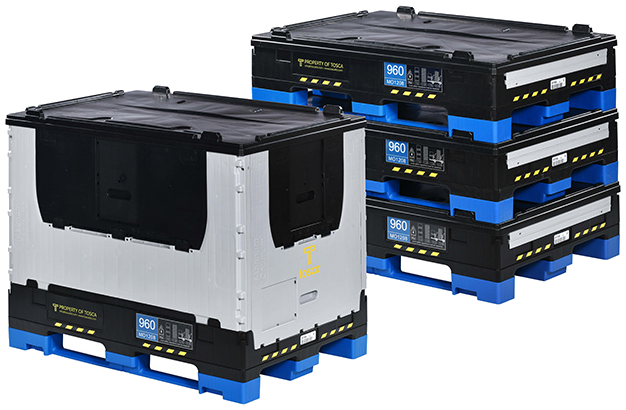
\includegraphics[width=0.4\linewidth]{figures/Magnum-Optimum_12108-removebg-preview.png}
  \caption{Full and empty folded RTIs}
  \label{fig:stacked-rti}
\end{figure}

\begin{figure}[h]
    \centering
        \resizebox{0.75\linewidth}{!}{\begin{tikzpicture}[
    % Define styles for consistent styling
    factory node/.style={
        circle,
        draw,
        minimum size=4.5cm,
        align=center,
        thick,
        fill=white
    },
    arrow/.style={
        -{Stealth[length=3mm, width=2mm]},
        thick
    },
    label text/.style={
        font=\sffamily,
        fill=white, % Adds a white background behind the text to break the line
        inner sep=4pt
    },
    plan text/.style={
        align=center, 
        font=\sffamily\small
    }
]

% -----------------------------------------
% 1. Main Circular Nodes (Plant & Supplier)
% -----------------------------------------
\node[factory node] (plant) at (0,0) {
    \includesvg[width=1.5cm]{figures/factory.svg}\\[0.3cm]
    Plant
};

\node[factory node] (supplier) at (14,0) {
    \includesvg[width=1.5cm]{figures/factory.svg}\\[0.3cm]
    Supplier
};

% -----------------------------------------
% 2. Curved Routing Arrows (Top & Bottom)
% -----------------------------------------
% Supplier -> Plant (Top)
\draw[arrow] (supplier) to[bend right=20] 
    node[label text] {Transport of full RTIs} (plant);

% Plant -> Supplier (Bottom)
\draw[arrow] (plant) to[bend right=20] 
    node[label text] {Transport of empty RTIs} (supplier);

% -----------------------------------------
% 3. Production Plan (Left side)
% -----------------------------------------
\node[plan text] (plan_left) at (-4, 0) {Production unloads \\ full RTIS};
% Arrows pointing to Plant
\draw[arrow] (plan_left.east) -- ($(plant.west)+(0, 0.6)$);
\draw[arrow] (plan_left.east) -- ($(plant.west)-(0, 0.6)$);

% -----------------------------------------
% 4. Production Plan (Right side)
% -----------------------------------------
\node[plan text] (plan_right) at (18, 0) {Production loads \\ empty RTIs};
% Arrows pointing to Supplier
\draw[arrow] (plan_right.west) -- ($(supplier.east)+(0, 0.6)$);
\draw[arrow] (plan_right.west) -- ($(supplier.east)-(0, 0.6)$);

\end{tikzpicture}
}
    \caption{ One-to-one RTI return strategy }
\label{fig:1to1RTI}
\end{figure}

When a central decision-maker, such as a dominant tier-1 manufacturer, an original equipment manufacturer (OEM) that owns the RTI pool, or a SC platform acting as manufacturing as a service (MaaS) {\color{red} Add reference}, has visibility over the entire network, a collaborative RTI return strategy becomes possible. Rather than using a one-to-one RTI return strategy, the model optimizes empty RTI routes, reducing the total distance an empty RTI journeys and consolidating routes. This simultaneously diminishes RTI return costs and the overall RTI pool size. Figure~\ref{fig:sc1to1} shows the one-to-one baseline, while Figure \ref{fig:scshared} illustrates how an optimized collaborative strategy reduces RTI return transport costs on the same network. Determining the service network design is the primary objective of this research.

\begin{figure}[H]
    \centering
    \begin{subfigure}[b]{0.49\linewidth}
        \centering
        \resizebox{\linewidth}{!}{\begin{tikzpicture}

  \placeSCnodes

  %% ── Full RTI routes (black) ───────────────────────────────────────────────
  \draw[routefull] (A) -- (B)
    node[midway, below=3pt, font=\scriptsize\bfseries]{10};
  \draw[routefull] (B) -- (C)
    node[midway, right=3pt, font=\scriptsize\bfseries]{15};
  \draw[routefull] (D) -- (A)
    node[midway, left=3pt,  font=\scriptsize\bfseries]{10};
  \draw[routefull] (E) -- (F)
    node[midway, right=3pt, font=\scriptsize\bfseries]{10};

  %% ── Empty RTI return routes (blue, slight offset) ─────────────────────────
  \draw[routeempty, transform canvas={yshift= 4pt}]
    (B) -- (A) node[midway, above=1pt, font=\scriptsize\bfseries, color=blue!70]{10};
  \draw[routeempty, transform canvas={xshift=-4pt}]
    (C) -- (B) node[midway, left=1pt,  font=\scriptsize\bfseries, color=blue!70]{15};
  \draw[routeempty, transform canvas={xshift= 4pt}]
    (A) -- (D) node[midway, right=1pt, font=\scriptsize\bfseries, color=blue!70]{10};
  \draw[routeempty, transform canvas={yshift= 4pt}]
    (F) -- (E) node[midway, above=1pt, font=\scriptsize\bfseries, color=blue!70]{10};

%% ── Legend ────────────────────────────────────────────────────────────────
  \begin{scope}[shift={(\legendCoord)}]
    \node[scnode] (ln) at (0, 0) {};
    \node[right=0.1cm of ln, font=\scriptsize, text width=2.4cm] {SC nodes};
    
    \draw[routefull]  (-0.2, -0.6) -- (0.8, -0.6)
      node[right, font=\scriptsize] {Routes of full RTIs};
      
    \draw[routeempty] (-0.2, -1.2) -- (0.8, -1.2)
      node[right, font=\scriptsize] {Return of empty RTIs};
  \end{scope}



\end{tikzpicture}
}
        \caption{\textit{One-to-one} relationship}
        \label{fig:sc1to1}
    \end{subfigure}
    \hfill
    \begin{subfigure}[b]{0.45\linewidth}
        \centering
        \resizebox{\linewidth}{!}{\begin{tikzpicture}

  \placeSCnodes

  %% ── Full RTI routes (black) ───────────────────────────────────────────────
  \draw[routefull] (A) -- (B)
    node[midway, above=2pt, font=\scriptsize\bfseries]{10};
  \draw[routefull] (B) -- (C)
    node[midway, right=3pt, font=\scriptsize\bfseries]{15};
  \draw[routefull] (D) -- (A)
    node[midway, left=3pt,  font=\scriptsize\bfseries]{10};
  \draw[routefull] (E) -- (F)
    node[midway, right=3pt, font=\scriptsize\bfseries]{10};

  %% ── Optimised empty-RTI return routes (blue) ──────────────────────────────
  % C sends 5 empties back up to B
  \draw[routeempty, transform canvas={xshift=-4pt}]
    (C) -- (B) node[midway, left=1pt, font=\scriptsize\bfseries, color=blue!70]{5};

  % C sends 10 empties sideways to E (shared consolidation)
  \draw[routeempty] (C) -- (E)
    node[midway, above=2pt, font=\scriptsize\bfseries, color=blue!70]{10};

  % D sends 10 empties up to A  (consolidated leg)
  \draw[routeempty, transform canvas={xshift=1pt}]
    (F) -- (D) node[midway, right, font=\scriptsize\bfseries, color=blue!70]{10};

%% ── Legend ────────────────────────────────────────────────────────────────
  \begin{scope}[shift={(\legendCoord)}]
    \node[scnode] (ln) at (0, 0) {};
    \node[right=0.1cm of ln, font=\scriptsize, text width=2.4cm] {SC nodes};
    
    \draw[routefull]  (-0.2, -0.6) -- (0.8, -0.6)
      node[right, font=\scriptsize] {Routes of full RTIs};
      
    \draw[routeempty] (-0.2, -1.2) -- (0.8, -1.2)
      node[right, font=\scriptsize] {Routes of empty RTIs};
  \end{scope}
\end{tikzpicture}



}
        \caption{SND with minimized RTI return transport cost}
        \label{fig:scshared}
    \end{subfigure}
    \caption{SND with minimized RTI return transport cost}
\end{figure}

On certain routes, full RTIs are accompanied by protective accessories,
such as nets or lids, that secure parts during transit. These
\textit{inlays} are themselves reusable and must be returned to the origin
site after unloading. Here the FTL and LTL, also known as groupage, transport modes are addressed. 

The model takes as input data the average daily flows of full RTIs between nodes, derived from released production plans over a planning horizon chosen by the decision-maker, typically a month, quarter, or year. These averages are assumed to be representative of the considered planning horizon, meaning that demands are sufficiently stable for the average to serve as reliable input data, without extreme imbalances that would render it misleading. 

{\color{blue}
While the physical routing of full RTIs is set in advance by established production and procurement contracts (i.e., a specific supplier must deliver to a specific customer a given set of products), the logistical execution of these forward flows is subject to optimization. Specifically, the model determines two operational parameters for the forward flows. First, it selects the optimal RTI type from a set of compatible options for each product. This selection affects the required transport capacity and the subsequent volume of empty returns, as different RTI types possess distinct dimensions and folding ratios. Second, the model determines the dispatch frequency for these full shipments. The shipment frequency governs the accumulation of inventory, creating a fundamental trade-off: longer intervals between shipments improve vehicle utilization and reduce fixed transport costs, but need a larger RTI pool to cover in-transit and waiting stock. Consequently, minimizing the total system cost requires the joint optimization of forward dispatch frequencies and packaging types, alongside the consolidation of empty return routes.
}

Under this assumption, the problem can be considered a service network design for RTIs, which consists of finding the tradeoff among daily RTI transport cost, which include transport costs for both full and empty RTIs; the inventory holding cost of the RTI pool; and CO$_2$ emissions from RTI transport. The model determines:

\begin{enumerate}
  \item Routes for empty RTI and inlay return flows.
  \item The RTI type selection for products with multiple compatible packaging options.
  \item The shipment frequency per route (both full and empty flows), expressed as a \textit{queue time} (Q-day), i.e.\ the number of days between consecutive dispatches.
  \item The transport mode per route, i.e. FTL or LTL.
  \item The total number of RTIs needed in the whole SC network.
\end{enumerate}

% ─────────────────────────────────────────────────────────────────
The problem encompasses a strategic-tactical decision level, using as input data the daily averages of RTI demand flows. In practice, the daily average flow of full RTIs between nodes is managed by medium-to-long-term production contracts and procurement agreements, which should remain stable over the planning horizon under consideration. The Q-days and transport modes are likewise set with a medium-to-long-term frequency rather than renegotiated daily or weekly. By optimizing strategic-tactical decisions for a given planning horizon, instead of multi-period decisions, the model is computationally efficient even for large industrial networks, where a fully operational multi-period optimization could be intractable to solve. Here, the strategic-tactical perspective provides a scalable upper bound on the achievable savings from collaborative RTI management, by establishing transport routes, Q-days and the RTI pool size, which can subsequently serve as input data for operational-level RTI transport planning.


Given:
\begin{itemize}
    \item Flow of full RTIs across the supply chain.
    \item Safety Stocks of the supply chain nodes.
    \item Economic and environmental Transport Costs across the supply chain.
\end{itemize}


To determine:

 \begin{itemize}
     \item Transport decisions, including routes and method of transport.
     \item Number of RTIs needed in the network.
 \end{itemize}

 

KPIs: One to One comparison. 
% 
\section{Mathematical Model}

\begin{longtable}{|p{0.19\textwidth}|p{0.8\textwidth}|}
\caption{Model nomenclature}
\label{tab:nomenclature}\\
\hline
\multicolumn{2}{|l|}{\textbf{Indices and Sets}}\\ \hline
$V$ & Set of nodes representing manufacturing plants, $i, j \in V$ \\
$E$ & Set of directed edges representing potential transport lanes,
      $E \subseteq V \times V$ \\
\hline
\multicolumn{2}{|l|}{\textbf{Parameters}}\\ \hline
$\mu_{ij}$     & Daily average number of full RTIs shipped from node $i$
                 to node $j$, $(i,j)\in E$ \\
$ric_{ij}$     & Fraction of full RTI shipments on lane $(i,j)$ that
                 require a return inlay \\
$c^{f}_{ij}$,\ $c^{e}_{ij}$ & Unit transport cost per RTI on lane $(i,j)$
                 for full and empty flows, respectively \\
$M$            & Sufficiently large constant (big-M) \\
\hline
\multicolumn{2}{|l|}{\textbf{Decision Variables}}\\ \hline
\multicolumn{2}{|l|}{\textit{Binary variables}}\\ \hline
$X_{ij}$  & 1 if lane $(i,j)$ is active for any RTI flow, 0 otherwise \\
$XF_{ij}$ & 1 if lane $(i,j)$ carries full RTIs, 0 otherwise \\
$XI_{ij}$ & 1 if lane $(i,j)$ carries return inlays, 0 otherwise \\
$XE_{ij}$ & 1 if lane $(i,j)$ carries empty RTIs, 0 otherwise \\
\hline
\multicolumn{2}{|l|}{\textit{Flow variables}}\\ \hline
$NF_{ij}$ & Daily average number of full RTIs sent from $i$ to $j$ \\
$NI_{ij}$ & Daily average number of return inlays sent from $i$ to $j$ \\
$NE_{ij}$ & Daily average number of empty RTIs sent from $i$ to $j$ \\
\hline
\multicolumn{2}{|l|}{\textit{Cost variables}}\\ \hline
$CF_{ij}$,\ $CI_{ij}$,\ $CE_{ij}$ & Daily transport cost on lane $(i,j)$
                 for full RTIs, return inlays, and empty RTIs, respectively \\
\hline
\end{longtable}

The objective minimises the total daily transport cost across all lanes and
flow types:

%
\begin{align}
  \min \quad & \sum_{(i,j)\in E}
    \bigl(CF_{ij} + CI_{ij} + CE_{ij}\bigr)
  \label{eq:objective}
\end{align}

\paragraph{Daily transport costs.}
The daily transport cost on each lane is defined for each flow type. Full RTIs
and return inlays share the same unit cost, as inlays travel consolidated with
full shipments; empty RTIs are charged at their own rate:
%
\begin{align}
  CF_{ij} &= NF_{ij}\cdot c^{f}_{ij}
    && \forall\,(i,j)\in E
    \label{eq:cost-full}\\
  CI_{ij} &= NI_{ij}\cdot c^{f}_{ij}
    && \forall\,(i,j)\in E
    \label{eq:cost-inlay}\\
  CE_{ij} &= NE_{ij}\cdot c^{e}_{ij}
    && \forall\,(i,j)\in E
    \label{eq:cost-empty}
\end{align}

\paragraph{Flow conservation.}
The total number of RTIs entering each node must equal the total number leaving
it, ensuring a closed-loop network:
%
\begin{align}
  \sum_{j \in V}\!\bigl(NE_{ij}+NF_{ij}+NI_{ij}\bigr)
  &= \sum_{j \in V}\!\bigl(NE_{ji}+NF_{ji}+NI_{ji}\bigr)
  && \forall\, i \in V
  \label{eq:flow-conservation}
\end{align}

\paragraph{Fixed full-RTI and inlay flows.}
Full RTI flows are determined by production plans and are therefore treated as
input parameters. Return inlays must be sent back on the reverse lane in
proportion to the full shipments that required them:
%
\begin{align}
  NF_{ij} &= \mu_{ij}
    && \forall\,(i,j) \in E
    \label{eq:full-flow-fixed} \\
  NI_{ji} &= ric_{ij}\cdot\mu_{ij}
    && \forall\,(i,j) \in E
    \label{eq:inlay-flow-fixed}
\end{align}

\paragraph{Lane activation.}
A lane is considered active if and only if it carries at least one type of RTI
flow. The aggregate activation variable $X_{ij}$ is linked to the
type-specific variables as follows:
%
\begin{align}
  X_{ij} &\geq XF_{ij},\quad
  X_{ij} \geq XI_{ij},\quad
  X_{ij} \geq XE_{ij}
    && \forall\,(i,j) \in E
    \label{eq:lane-activation-lb} \\
  X_{ij} &\leq XF_{ij} + XI_{ij} + XE_{ij}
    && \forall\,(i,j) \in E
    \label{eq:lane-activation-ub}
\end{align}

\paragraph{Flow--binary consistency.}
Each type-specific binary variable is active if and only if a positive flow
of the corresponding RTI type is present on that lane:
%
\begin{align}
  NF_{ij} &\leq M\cdot XF_{ij}
    && \forall\,(i,j) \in E
    \label{eq:bigM-full} \\
  NI_{ij} &\leq M\cdot XI_{ij}
    && \forall\,(i,j) \in E
    \label{eq:bigM-inlay} \\
  NE_{ij} &\leq M\cdot XE_{ij}
    && \forall\,(i,j) \in E
    \label{eq:bigM-empty} \\[4pt]
  XF_{ij} &\leq NF_{ij}
    && \forall\,(i,j) \in E
    \label{eq:lb-full} \\
  XI_{ij} &\leq NI_{ij}
    && \forall\,(i,j) \in E
    \label{eq:lb-inlay} \\
  XE_{ij} &\leq NE_{ij}
    && \forall\,(i,j) \in E
    \label{eq:lb-empty}
\end{align}


% \section{Mathematical Model}

\begin{longtable}{|p{0.20\textwidth}|p{0.79\textwidth}|}
\caption{Model nomenclature}
\label{tab:nomenclature}\\
\hline
\multicolumn{2}{|l|}{\textbf{Indices and Sets}}\\ \hline
$V$          & Set of nodes representing manufacturing plants, $i,j \in V$ \\
$E$          & Set of directed edges representing potential transport lanes,
               $E \subseteq V \times V$ \\
$C$          & Set of RTI types, $c \in C$ \textit{(to be incorporated)} \\
\hline
\multicolumn{2}{|l|}{\textbf{Parameters}}\\ \hline
$\mu_{ij}$        & Daily average number of full RTIs shipped on lane $(i,j)$ \\
$ric_{ij}$        & Fraction of full shipments on lane $(i,j)$ that require a
                    return inlay \\
$c_{ij}$          & Transport cost per unit volume on lane $(i,j)$ \\
$f_{ij}$          & Fixed cost per shipment on lane $(i,j)$ \\
$v^{f}$, $v^{e}$  & Volume occupied by one full and one empty RTI,
                    respectively \\
$l_{ij}$          & Transit time on lane $(i,j)$, in days \\
$\alpha^{f}$, $\alpha^{e}$ & Maintenance loss factor for full and empty RTIs,
                    respectively \\
$ssf^{i}_{ij}$, $ssf^{j}_{ij}$ & Safety stock of full RTIs held at the origin
                    and destination node of lane $(i,j)$ \\
$sse^{i}_{ij}$, $sse^{j}_{ij}$ & Safety stock of empty RTIs held at the origin
                    and destination node of lane $(i,j)$ \\
$s^{\text{RTI}}$  & Initial RTI pool available before optimisation \\
$p^{\text{RTI}}$  & Unit purchase cost of one RTI \\
$\omega_{ij}$     & Minimum shipment volume on lane $(i,j)$ \\
$\delta_{ij}$     & Maximum shipment volume on lane $(i,j)$ \\
$M$               & Sufficiently large constant (big-$M$) \\
\hline
\multicolumn{2}{|l|}{\textbf{Decision Variables}}\\ \hline
\multicolumn{2}{|l|}{\textit{Binary variables}}\\ \hline
$X_{ij}$     & 1 if lane $(i,j)$ is active for any RTI flow, 0 otherwise \\
$XF_{ij}$    & 1 if lane $(i,j)$ carries full RTIs, 0 otherwise \\
$XI_{ij}$    & 1 if lane $(i,j)$ carries return inlays, 0 otherwise \\
$XE_{ij}$    & 1 if lane $(i,j)$ carries empty RTIs, 0 otherwise \\
\hline
\multicolumn{2}{|l|}{\textit{Daily flow variables}}\\ \hline
$NF_{ij}$    & Daily average number of full RTIs sent from $i$ to $j$ \\
$NI_{ij}$    & Daily average number of return inlays sent from $i$ to $j$ \\
$NE_{ij}$    & Daily average number of empty RTIs sent from $i$ to $j$ \\
\hline
\multicolumn{2}{|l|}{\textit{Daily volume variables}}\\ \hline
$VF_{ij}$    & Daily volume of full RTIs on lane $(i,j)$ \\
$VI_{ij}$    & Daily volume of return inlays on lane $(i,j)$ \\
$VE_{ij}$    & Daily volume of empty RTIs on lane $(i,j)$ \\
\hline
\multicolumn{2}{|l|}{\textit{Per-shipment variables}}\\ \hline
$q_{ij}$     & Queue time on lane $(i,j)$: days between consecutive
               dispatches (continuous, $q_{ij} \geq 1$) \\
$VS_{ij}$    & Total volume per shipment on lane $(i,j)$
               [$= (VF_{ij}+VI_{ij}+VE_{ij})\cdot q_{ij}$,\ \textit{bilinear}] \\
$NSF_{ij}$, $NSI_{ij}$, $NSE_{ij}$ & Number of full, inlay and empty RTIs
               per shipment on lane $(i,j)$
               [$= NF_{ij}\cdot q_{ij}$, etc.,\ \textit{bilinear}] \\
\hline
\multicolumn{2}{|l|}{\textit{Total RTI pool variables}}\\ \hline
$TNCF_{ij}$  & Total full RTIs allocated to lane $(i,j)$, accounting for
               in-transit stock, safety stock, and maintenance losses \\
$TNCI_{ij}$  & Total inlay RTIs allocated to lane $(i,j)$ \\
$TNCE_{ij}$  & Total empty RTIs allocated to lane $(i,j)$, accounting for
               in-transit stock, safety stock, and maintenance losses \\
$P$          & Number of additional RTIs to purchase ($P \geq 0$) \\
\hline
\multicolumn{2}{|l|}{\textit{Cost variables}}\\ \hline
$CF_{ij}$    & Daily transport cost of full RTIs on lane $(i,j)$ \\
$CI_{ij}$    & Daily transport cost of return inlays on lane $(i,j)$ \\
$CE_{ij}$    & Daily transport cost of empty RTIs on lane $(i,j)$ \\
$TC_{ij}$    & Total daily transport cost on lane $(i,j)$ \\
$TCS_{ij}$   & Transport cost per shipment on lane $(i,j)$
               [$= VS_{ij}\cdot c_{ij} + X_{ij}\cdot f_{ij}$] \\
\hline
\end{longtable}

% ─────────────────────────────────────────────────────────────────
\paragraph{Objective function.}
Minimise the total daily transport cost across all lanes plus the amortised
purchase cost of any additional RTIs required:
%
\begin{align}
  \min \quad \sum_{(i,j)\in E} TC_{ij} \;+\; p^{\text{RTI}} \cdot P
  \label{eq:objective}
\end{align}

% ─────────────────────────────────────────────────────────────────
\paragraph{Flow conservation.}
The total number of RTIs entering each node equals the total number leaving it,
ensuring a closed-loop network:
%
\begin{align}
  \sum_{j \in V}\!\bigl(NE_{ij}+NF_{ij}+NI_{ij}\bigr)
  &= \sum_{j \in V}\!\bigl(NE_{ji}+NF_{ji}+NI_{ji}\bigr)
  && \forall\, i \in V
  \label{eq:flow-conservation}
\end{align}

% ─────────────────────────────────────────────────────────────────
\paragraph{Fixed full-RTI and inlay flows.}
Full RTI flows are fixed by production plans. Return inlays are sent back on
the reverse lane in proportion to the full shipments that required them:
%
\begin{align}
  NF_{ij} &= \mu_{ij}
    && \forall\,(i,j)\in E
    \label{eq:full-fixed}\\
  NI_{ji} &= ric_{ij}\cdot\mu_{ij}
    && \forall\,(i,j)\in E
    \label{eq:inlay-fixed}
\end{align}

% ─────────────────────────────────────────────────────────────────
\paragraph{Lane activation.}
A lane is active if and only if it carries at least one RTI flow type:
%
\begin{align}
  X_{ij} &\geq XF_{ij}, \quad X_{ij} \geq XI_{ij}, \quad X_{ij} \geq XE_{ij}
    && \forall\,(i,j)\in E
    \label{eq:activation-lb}\\
  X_{ij} &\leq XF_{ij} + XI_{ij} + XE_{ij}
    && \forall\,(i,j)\in E
    \label{eq:activation-ub}
\end{align}

% ─────────────────────────────────────────────────────────────────
\paragraph{Flow--binary consistency.}
Each binary is active if and only if a positive flow of the corresponding type
is present:
%
\begin{align}
  NF_{ij} &\leq M\cdot XF_{ij}, \quad XF_{ij} \leq NF_{ij}
    && \forall\,(i,j)\in E
    \label{eq:binary-full}\\
  NI_{ij} &\leq M\cdot XI_{ij}, \quad XI_{ij} \leq NI_{ij}
    && \forall\,(i,j)\in E
    \label{eq:binary-inlay}\\
  NE_{ij} &\leq M\cdot XE_{ij}, \quad XE_{ij} \leq NE_{ij}
    && \forall\,(i,j)\in E
    \label{eq:binary-empty}
\end{align}

% ─────────────────────────────────────────────────────────────────
\paragraph{Daily volumes.}
The daily volume on each lane is determined by the number of RTIs and their
individual volumes:
%
\begin{align}
  VF_{ij} &= NF_{ij}\cdot v^{f}
    && \forall\,(i,j)\in E
    \label{eq:vol-full}\\
  VI_{ij} &= NI_{ij}\cdot v^{f}
    && \forall\,(i,j)\in E
    \label{eq:vol-inlay}\\
  VE_{ij} &= NE_{ij}\cdot v^{e}
    && \forall\,(i,j)\in E
    \label{eq:vol-empty}
\end{align}

% ─────────────────────────────────────────────────────────────────
\paragraph{Per-shipment quantities.}
The number of RTIs and total volume accumulated between consecutive dispatches
are proportional to the queue time. These constraints are \emph{bilinear} and
will be linearised in Section~\ref{sec:linearisation}:
%
\begin{align}
  NSF_{ij} &= NF_{ij}\cdot q_{ij}
    && \forall\,(i,j)\in E
    \label{eq:ship-full}\\
  NSI_{ij} &= NI_{ij}\cdot q_{ij}
    && \forall\,(i,j)\in E
    \label{eq:ship-inlay}\\
  NSE_{ij} &= NE_{ij}\cdot q_{ij}
    && \forall\,(i,j)\in E
    \label{eq:ship-empty}\\
  VS_{ij}  &= \bigl(VF_{ij}+VI_{ij}+VE_{ij}\bigr)\cdot q_{ij}
    && \forall\,(i,j)\in E
    \label{eq:ship-vol}
\end{align}

% ─────────────────────────────────────────────────────────────────
\paragraph{Shipment volume bounds.}
Each shipment must respect a minimum load and a maximum vehicle capacity:
%
\begin{align}
  \omega_{ij}\cdot X_{ij} &\leq VS_{ij} \leq \delta_{ij}\cdot X_{ij}
    && \forall\,(i,j)\in E
    \label{eq:vol-bounds}
\end{align}

% ─────────────────────────────────────────────────────────────────
\paragraph{Total RTI pool requirements.}
The total number of RTIs allocated to each lane accounts for in-transit stock,
safety stock at both endpoints, and a maintenance loss factor:
%
\begin{align}
  TNCF_{ij} &= (1+\alpha^{f})\bigl(NSF_{ij} + l_{ij}\cdot NF_{ij}
               + XF_{ij}(ssf^{i}_{ij}+ssf^{j}_{ij})\bigr)
    && \forall\,(i,j)\in E
    \label{eq:pool-full}\\
  TNCE_{ij} &= (1+\alpha^{e})\bigl(NSE_{ij} + l_{ij}\cdot NE_{ij}
               + XE_{ij}(sse^{i}_{ij}+sse^{j}_{ij})\bigr)
    && \forall\,(i,j)\in E
    \label{eq:pool-empty}\\
  TNCI_{ij} &= (1+\alpha^{f})\bigl(NSI_{ij} + l_{ij}\cdot NI_{ij}\bigr)
    && \forall\,(i,j)\in E
    \label{eq:pool-inlay}
\end{align}

\paragraph{RTI purchase.}
Additional RTIs must be purchased to cover any shortfall between the network's
total requirement and the existing pool. If the existing pool is sufficient,
no purchase is needed and the surplus remains idle:
%
\begin{align}
  \sum_{(i,j)\in E}\bigl(TNCF_{ij}+TNCE_{ij}+TNCI_{ij}\bigr)
    &\leq s^{\text{RTI}} + P
    && P \geq 0
  \label{eq:purchase}
\end{align}

% ─────────────────────────────────────────────────────────────────
\paragraph{Daily transport costs.}
The per-shipment cost is the sum of a variable volumetric component and a fixed
dispatch cost. Dividing by the queue time converts it to a daily cost. This
constraint is \emph{bilinear} and will be linearised in
Section~\ref{sec:linearisation}:
%
\begin{align}
  TCS_{ij} &= VS_{ij}\cdot c_{ij} + X_{ij}\cdot f_{ij}
    && \forall\,(i,j)\in E
    \label{eq:cost-per-ship}\\
  TC_{ij}\cdot q_{ij} &= TCS_{ij}
    && \forall\,(i,j)\in E
    \label{eq:cost-daily}
\end{align}
:while
\section{Model Formulation}
% ══════════════════════════════════════════════════════════════════
%  NOTATION CONVENTION
% ══════════════════════════════════════════════════════════════════

Table \ref{tab:nomenclature} defines the sets, paramaters and variables of the model.

% ══════════════════════════════════════════════════════════════════
%  NOMENCLATURE
% ══════════════════════════════════════════════════════════════════

\begin{longtable}{|p{0.24\textwidth}|p{0.72\textwidth}|}
\caption{Model nomenclature}
\label{tab:nomenclature}\\
\hline
\multicolumn{2}{|l|}{\textbf{Indices and sets}}\\ \hline
$V$
  & Set of nodes representing manufacturing plants; $i,j\in V$ \\
$E\subseteq V\times V$
  & Set of directed edges representing potential transport routes \\
$R$
  & Set of RTI types; $r\in R$ \\
$\mathcal{M}$
  & Set of transport modes; $m\in\mathcal{M}$ \\
$H\subseteq V$
  & Set of hub nodes \\ \hline
\multicolumn{2}{|l|}{\textbf{Parameters}}\\ \hline
$\mu_{ijmpr}$
  & Daily average demand on route $(i,j)$ by mode $m$, product $p$,
    RTI type $r$; expressed in full RTI units \\
$ric_{ijpr}$
  & Fraction of full shipments on route $(i,j)$ of product $p$ in
    RTI type $r$ that require a return inlay; independent of
    transport mode \\
$bf_{ijmrp}$
  & 1 if full RTIs of type $r$ for product $p$ may traverse route
    $(i,j)$ by mode $m$; 0 otherwise \\
$be_{ijmr}$
  & 1 if empty RTIs of type $r$ may traverse route $(i,j)$ by
    mode $m$; 0 otherwise \\
$bm_{ijm}$
  & 1 if mode $m$ is available on route $(i,j)$; 0 otherwise \\
$bp_{ijp}$
  & 1 if product $p$ must be transported on route $(i,j)$;
    0 otherwise \\
$c_{ijm}$
  & Variable transport cost per unit volume on route $(i,j)$ by
    mode $m$ \\
$f_{ijm}$
  & Fixed dispatch cost per shipment on route $(i,j)$ by mode $m$ \\
$v^{f},\;v^{e}$
  & Volume occupied by one full (or inlay) RTI and one empty RTI,
    respectively \\
$l_{ijm}$
  & Transit time on route $(i,j)$ by mode $m$, in days \\
$q^{\min}_{m},\;q^{\max}_{m}$
  & Minimum and maximum queue time for mode $m$, in days \\
$\alpha^{f},\;\alpha^{e}$
  & Maintenance loss factor applied to full/inlay and empty RTIs,
    respectively \\
$ssf^{i}_{ijpr},\;ssf^{j}_{ijpr}$
  & Safety stock of full RTIs of type $r$ for product $p$ held at
    the origin and destination of route $(i,j)$, respectively;
    independent of transport mode \\
$sse^{i}_{ijpr},\;sse^{j}_{ijpr}$
  & Safety stock of empty RTIs of type $r$ for product $p$ held at
    the origin and destination of route $(i,j)$, respectively;
    independent of transport mode \\
$\omega_{ijm},\;\delta_{ijm}$
  & Minimum and maximum shipment volume on route $(i,j)$ by
    mode $m$ \\
$fhc_{i},\;vhc_{i}$
  & Fixed activation cost and variable cost per unit volume at
    hub $i\in H$, respectively \\
$s^{\text{RTI}}_{r}$
  & Existing pool of RTI type $r$ available before optimisation \\
$p^{\text{RTI}}_{r}$
  & Unit purchase cost of one RTI of type $r$ \\
$M$
  & Sufficiently large constant (big-$M$) \\ \hline
\multicolumn{2}{|l|}{\textbf{Decision variables --- binary}}\\ \hline
$X_{ijmr}$
  & 1 if route $(i,j)$ carries any RTIs of type $r$ for product $p$
    by mode $m$; 0 otherwise \\
$XF_{ijmpr}$, $\;XI_{ijmr}$, $\;XE_{ijmr}$
  & 1 if route $(i,j)$ carries full RTIs, return inlays, or empty
    RTIs (resp.) of type $r$ for product $p$ by mode $m$;
    0 otherwise \\
$XH_{i}$
  & 1 if hub $i\in H$ is activated; 0 otherwise \\ \hline
\multicolumn{2}{|l|}{\textbf{Decision variables --- daily flow}}\\ \hline
$N_{ijmr}$, $\;NF_{ijmpr}$, $\;NI_{ijmr}$, $\;NE_{ijmr}$
  & Daily average number of RTIs (total), full RTIs, return inlays,
    and empty RTIs on route $(i,j)$, respectively \\
$V_{ijmr}$, $\;VF_{ijmpr}$, $\;VI_{ijmr}$, $\;VE_{ijmr}$
  & Daily average volume of RTIs (total), full RTIs, return inlays,
    and empty RTIs on route $(i,j)$, respectively \\ \hline
\multicolumn{2}{|l|}{\textbf{Decision variables --- per shipment}}\\ \hline
$q_{ijm}$
  & Queue time on route $(i,j)$ by mode $m$: days between
    consecutive dispatches \\
$NS_{ijmr}$, $\;NSF_{ijmr}$, $\;NSI_{ijmr}$, $\;NSE_{ijmr}$
  & Total number of RTIs (total), full RTIs, return inlays, and
    empty RTIs loaded per shipment on route $(i,j)$ \\
$VS_{ijmr}$, $\;VSF_{ijmr}$, $\;VSI_{ijmr}$, $\;VSE_{ijmr}$
  & Total volume (total), full RTI volume, inlay volume, and empty
    RTI volume per shipment on route $(i,j)$ \\ \hline
\multicolumn{2}{|l|}{\textbf{Decision variables --- RTI pool}}\\ \hline
$TNC_{ijmr}$, $\;TNCF_{ijmr}$, $\;TNCE_{ijmr}$, $\;TNCI_{ijmr}$
  & RTIs (total), full RTIs, empty RTIs, and inlay RTIs allocated
    to route $(i,j)$, covering queue stock, in-transit stock,
    safety stock, and losses \\
$P_{r}$
  & Additional RTIs of type $r$ to purchase; $P_{r}\geq 0$ \\ \hline
\multicolumn{2}{|l|}{\textbf{Decision variables --- cost and hub}}\\ \hline
$TCS_{ijm}$
  & Transport cost per shipment on route $(i,j)$ by mode $m$ \\
$TC_{ijm}$
  & Daily transport cost on route $(i,j)$ by mode $m$ \\
$VH_{i}$
  & Total daily volume handled at hub $i\in H$ \\
$CH_{i}$
  & Daily handling cost at hub $i\in H$ \\ \hline
\end{longtable}

\begin{convention}[Index suppression and aggregation from the root variable]
\label{conv:notation}

Every variable in the model is defined with a given root indices. For example, variable $\phi$, is defined with the following indices $(c\in C,i\in V,j\in V,m\in \mathcal{M})$; we call this the \textbf{root variable}.
Writing a variable with fewer indices always denotes a
\emph{derived variables}: one or more indices have been suppressed and
the root values aggregated according to the rules below.



% ------------------------------------------------------------------
\medskip
\noindent\textbf{Rule~1 (Sum aggregation).
 }

Dropping any indeces from any variable $\phi$ stands for the sum of
the root variables over every value of those indices:
%k
\begin{align*}
  \phi_{cij}
    &\;\coloneqq\; \sum_{m\in\mathcal{M}} \phi_{cijm},
  &
  \phi_{ijm}
    &\;\coloneqq\; \sum_{c\in C}           \phi_{cijm},
  &
  \phi
    &\;\coloneqq\;
      \sum_{c\in C}\sum_{i\in V}\sum_{j\in V}\sum_{m\in\mathcal{M}} \phi_{cijm}.
\end{align*}
%
For continuous and integer variables this is the natural
interpretation.
For binary variables the result is an \emph{integer count} of how
many root-level binaries in the group equal~1; it is not itself
binary.
For example, $X_{cij} \coloneqq \sum_{m\in\mathcal{M}}
X_{cijm}$ counts how many modes are active for type $c$ on
lane $(i,j)$ and takes values in $\{0,1,\dots,|\mathcal{M}|\}$.
The sum aggreagtion can be considered a shorthand notation, since we do not need to create new variables in the solver. We can also create derived $\phi$ variable to the model and the associated constraint.:while

% ------------------------------------------------------------------
\medskip
\noindent\textbf{Rule~2 (Dot notation for the node-pair $(i,j)$).}

The root variable carries two active indices from the same set $V$.
Suppressing one while keeping the other would be ambiguous, so a
dot~$(\,\cdot\,)$ marks the suppressed position explicitly:
%
\begin{align*}
  \phi_{c\cdot j m}
    &\;\coloneqq\; \sum_{i\in V} \phi_{cijm},
  &
  \phi_{ci \cdot m}
    &\;\coloneqq\; \sum_{j\in V} \phi_{cijm}.
\end{align*}
%
The dot is only ever needed for the origin/destination pair, as no
other pair of active indices belongs to the same set.
Rule~1 applies as normal: the result is a sum, and for binary
variables it is an integer count.

% ------------------------------------------------------------------
\medskip
\noindent\textbf{Rule~3 (OR-aggregated binaries).
  }

We can also aggregate binary variables to denote an OR aggreagtion. Then, a new binary decision variable is introduced,
denoted with an overline ($\overline{X}$).
This variable is not a notational shorthand: it must be declared
in the solver and its relationship to the root-level binaries
enforced by an explicit big-$M$ pair, or boolean imposition.
Crucially, the pair is written directly in terms of the
sum aggregate defined by Rule~1, so the sum-shorthand appears
in the constraints themselves.

\smallskip
\noindent\emph{Suppressing the mode index $m$} yields the new
binary $\overline{X}_{cij}$, linked to the sum aggregate
$X_{cij} = \sum_{m\in\mathcal{M}} X_{cijm}$ by:
%
\begin{align}
  \overline{X}_{cij}
    &\leq X_{cij}
  && \forall\,(i,j)\in E,\ c\in C
  \label{eq:or-m-lb}\\
  X_{cij}
    &\leq |M|\cdot\overline{X}_{cij}
  && \forall\,(i,j)\in E,\ c\in C
  \label{eq:or-m-ub}
\end{align}
%
Constraint~\eqref{eq:or-m-lb} forces $\overline{X}_{cij}$
to~0 when the count $X_{cij}$ is~0 (no mode active).
Constraint~\eqref{eq:or-m-ub} forces $\overline{X}_{cij}$
to~1 when the count is positive (at least one mode active).
Together they enforce
$\overline{X}_{cij} = 1 \iff X_{cij} \geq 1$.

% ------------------------------------------------------------------
\medskip
\noindent\textbf{Rule~4 (At Least One)}

We can also aggregate binary variables to denote an At Least One (ALO) aggreagtion. Then, a new binary decision variable is introduced,
denoted with an overline  $\overline{X}_{cij}$. We also need to
%
\begin{align}
  X_{cij}
    &= 1
  && \forall\,(i,j)\in E
  \label{eq:exactly-one}
\end{align}
%


% ------------------------------------------------------------------
%  TIKZ LATTICE
% ------------------------------------------------------------------
\begin{figure}[H]
\centering
\resizebox{0.95\linewidth}{!}{%
  % --- ADJUSTABLE PARAMETERS ---
\def\hsep{4.0}
\def\vsep{1.4}
\def\logicXshift{7.5}
% -----------------------------
\begin{tikzpicture}[
  every node/.style = {
    draw, rounded corners=3pt, inner sep=5pt,
    align=center, font=\small, thick
  },
  rootBox/.style   = {fill=blue!10, draw=blue!60!black},
  sumBox/.style    = {fill=orange!10, draw=orange!60!black},
  binBox/.style    = {fill=red!5, draw=red!80!black, dashed},
  arr/.style       = {->, >=stealth, thick},
  barr/.style      = {->, >=stealth, thick, dashed, red!80!black},
  lbl/.style       = {draw=none, fill=none, font=\footnotesize\itshape, inner sep=2pt},
  blbl/.style      = {draw=none, fill=none, font=\footnotesize\bfseries, inner sep=2pt, text=red!80!black},
  graylbl/.style   = {draw=none, fill=none, font=\small\bfseries, gray!50}
]

%% --- SUM AGGREGATION SECTION (Left) ---
\node[rootBox] (root) at (0,0) {$\phi_{cijm}$};
\node[sumBox] (Fcij)  at (-\hsep/2, \vsep)
  {$\widetilde{\phi}_{cij} \coloneqq \sum_{m \in \mathcal{M}} \phi_{cijm}$};
\node[sumBox] (Fijm)  at (\hsep/2, \vsep)
  {$\widetilde{\phi}_{ijm} \coloneqq \sum_{c \in C} \phi_{cijm}$};
\node[sumBox] (Fij)   at (0, 2*\vsep)
  {$\widetilde{\phi}_{ij} \coloneqq \sum_{c \in C} \sum_{m \in \mathcal{M}} \phi_{cijm}$};

\draw[arr] (root.north) -- (Fcij.south);
\draw[arr] (root.north) -- (Fijm.south);
\draw[arr] (Fcij.north) -- (Fij.south);
\draw[arr] (Fijm.north) -- (Fij.south);

% Dot notation
\node[sumBox] (dotj) at (-\hsep/2, -\vsep)
  {$\widetilde{\phi}_{c \cdot j m} \coloneqq \sum_{i \in V} \phi_{cijm}$};
\node[sumBox] (doti) at (\hsep/2, -\vsep)
  {$\widetilde{\phi}_{ci \cdot m} \coloneqq \sum_{j \in V} \phi_{cijm}$};

\draw[arr] (root.south) -- (dotj.north);
\draw[arr] (root.south) -- (doti.north);

%% --- BINARY LOGIC AGGREGATION SECTION (Right) ---
\begin{scope}[xshift=\logicXshift cm]
\node[rootBox] (Xroot) at (0, 0) {$X_{cijm}$};
\node[binBox] (XOR)  at (0, \vsep*1.36)
  {$\widecheck{X}_{cij}$ (OR aggregate) \\
   \scriptsize $\widecheck{X}_{cij} \leq \widetilde{X}_{cij}$ \\
   \scriptsize $\widetilde{X}_{cij} \leq |\mathcal{M}|\,\widecheck{X}_{cij}$};
\node[binBox] (XHAT) at (0, -\vsep*1.36)
  {$\widehat{X}_{cij}$ (At-most-one) \\
   \scriptsize $\widehat{X}_{cij} \leq \widetilde{X}_{cij}$ \\
   \scriptsize $\widetilde{X}_{cij} \leq \widehat{X}_{cij}$};

\draw[barr] (Xroot.north) -- (XOR.south)  node[blbl, midway, right] {Rule 3};
\draw[barr] (Xroot.south) -- (XHAT.north) node[blbl, midway, right] {Rule 4};
\end{scope}

%% --- DIVIDER AND LABELS ---
\draw[thick, gray!30, dashed]
  (\logicXshift/2, -1.5*\vsep) -- (\logicXshift/2, 2.8*\vsep);
\node[graylbl] at (0,            2.7*\vsep) {Sum Aggregation};
\node[graylbl] at (\logicXshift, 2.7*\vsep) {Binary Logic Aggregation};

\end{tikzpicture}
}
\caption{%
  Derivation lattice for a generic variable $\phi$ (left panel,
  continuous or integer) and its binary counterpart $X$ (right
  panel), separated by the dashed vertical rule.
  On the left, every arrow represents a sum aggregation
  (Rule~1--2): purely notational, no new variable introduced.
  On the right, solid arrows represent the same sum aggregation
  applied to binary variables, producing an integer count.
  Dashed arrows introduce a genuinely new solver variable (dashed
  border): the OR aggregate $\overline{X}$ (Rule~3), defined as a
  binary proxy for whether the count is positive, enforced by the
  big-$M$ pair shown in each node.
  The hat variant $\hat{X}$ (Rule~4) is the same variable as
  $\overline{X}_{cij}$ with the additional
  constraint~\eqref{eq:exactly-one} in force.%
}
\label{fig:index-lattice}
\end{figure}

\end{convention}



% ══════════════════════════════════════════════════════════════════
%  OBJECTIVE FUNCTION
% ══════════════════════════════════════════════════════════════════

\paragraph{Objective function.}
The model minimises three cost components: the total daily transport
cost across all routes and modes,
$\overline{TC}$;
the amortised purchase cost of any additional RTIs required to meet
pool requirements; and the total daily hub-handling cost
$CH$:
%
\begin{align}
  \min \quad
  \overline{TC}
  \;+\;
  \sum_{r\in R} p^{\text{RTI}}_{r} \cdot P_{r}
  \;+\;
  \overline{CH}.
  \label{eq:objective}
\end{align}

% ══════════════════════════════════════════════════════════════════
%  FLOW CONSERVATION
% ══════════════════════════════════════════════════════════════════

\paragraph{Flow conservation.}
RTIs circulate in a closed loop: the total daily outflow of RTI
type~$r$ from any node must equal its total daily inflow:
%
\begin{align}
  \overline{N}_{i\cdot r} &= \overline{N}_{\cdot i r}
  && \forall\,i\in V,\;r\in R,
  \label{eq:conservation}
\end{align}

% ══════════════════════════════════════════════════════════════════
%  FLOW--BINARY CONSISTENCY
% ══════════════════════════════════════════════════════════════════

\paragraph{Flow--binary consistency.}
Each root binary is active if and only if the corresponding
daily average flow is strictly positive, and only when the route
is physically permissible as encoded by the $b$-parameters:
%
\begin{align}
  NF_{ijmpr} &\leq M\cdot XF_{ijmpr},
  \quad
  XF_{ijmpr} \leq NF_{ijmpr}\cdot bf_{ijmpr}
  && \forall\,(i,j)\in E,\;m\in\mathcal{M},\;p,\;r\in R
  \label{eq:binary-full}\\
  NI_{ijmpr} &\leq M\cdot XI_{ijmpr},
  \quad
  XI_{ijmpr} \leq NI_{ijmpr}\cdot bf_{jimpr}
  && \forall\,(i,j)\in E,\;m\in\mathcal{M},\;p,\;r\in R
  \label{eq:binary-inlay}\\
  NE_{ijmr} &\leq M\cdot XE_{ijmr},
  \quad
  XE_{ijmr} \leq NE_{ijmr}\cdot be_{ijmr}
  && \forall\,(i,j)\in E,\;m\in\mathcal{M},\;p,\;r\in R.
  \label{eq:binary-empty} \\ 
  N_{ijmr} &= \overline{NF}_{ijmr}+\overline{NI}_{ijpr}+NE_{ijmr}
  && \forall\,(i,j)\in E,\;m\in\mathcal{M},\;p,\;r\in R. 
\end{align}

% ══════════════════════════════════════════════════════════════════
%  ROUTE ACTIVATION
% ══════════════════════════════════════════════════════════════════

\paragraph{Route activation.}
A route is active if and only if it carries at least one RTI
stream: full, empty, or inlay:
%
\begin{align}
  3\cdot X_{ijmr}
    &\geq \widecheck{XF}_{ijmr}+XE_{ijmr}+\widecheck{XI}_{ijmr}
  && \forall\,(i,j)\in E,\;m\in\mathcal{M},\;p,\;r\in R
  \label{eq:act-ub}\\
  X_{ijmr}
  &\leq  \widecheck{XF}_{ijmr}+XE_{ijmr}+\widecheck{XI}_{ijmr}
  && \forall\,(i,j)\in E,\;m\in\mathcal{M},\;p,\;r\in R.
  \label{eq:act-lb}
\end{align}

% ══════════════════════════════════════════════════════════════════
%  FULL-ROUTE ACTIVATION
% ══════════════════════════════════════════════════════════════════

\paragraph{Full-route activation.}
For any given product~$p$, at most one RTI type~$r$ may be used on
a given route. The at-most-one aggregate $\widehat{XF}_{ijp}$
 therefore equals~1 if and only if
product~$p$ is designated for route $(i,j)$, as encoded by the
binary parameter $bp_{ijp}$:
%
\begin{align}
  \widehat{XF}_{ijp} &= bp_{ijp}
  && \forall\,(i,j)\in E,\;p.
  \label{eq:full-activation}
\end{align}
This simultaneously enforces demand-driven activation and the
uniqueness of RTI type per product per route.

% ══════════════════════════════════════════════════════════════════
%  TRANSPORT MODE SELECTION
% ══════════════════════════════════════════════════════════════════

\paragraph{Transport mode selection.}
A mode may only be used on a route if it is physically available
there, and at most one mode may operate on any given route:
%
\begin{align}
  \widecheck{X}_{ijm}
    &\leqORIG bm_{ijm}
  && \forall\,(i,j)\in E,\;m\in\mathcal{M}
  \label{eq:mode-avail}\\
  \sum_{m\in\mathcal{M}} \widecheck{X}_{ijm}
    &\leq 1
  && \forall\,(i,j)\in E,
  \label{eq:mode-amo}
\end{align}

% ══════════════════════════════════════════════════════════════════
%  HUB NODES
% ══════════════════════════════════════════════════════════════════

\paragraph{Hub nodes.}
Hub nodes $i\in H\subseteq V$ are intermediate consolidation points
that aggregate outgoing flows and incur a handling cost with fixed
component $fhc_i\geq 0$ and variable component $vhc_i\geq 0$ per
unit volume.

At every non-hub node $i\in V\setminus H$, a node may not
simultaneously receive and dispatch empty RTIs of the same type $r\in R$:
%
\begin{align}
  \widecheck{XE}_{\cdot ir} + \widecheck{XE}_{i\cdot r}
    &\leq 1
  && \forall\,i\in V\setminus H, r\in R.
  \label{eq:hub-excl}
\end{align}
%
For every hub node $i\in H$, the binary $XH_i$ equals~1 if and
only if hub~$i$ is activated, i.e.\ if at least one outgoing route
from~$i$ is used:
%
\begin{align}
  XH_i &= \widecheck{X}_{i\cdot}
  && \forall,i\in H
  \label{eq:hub-XH}\\[4pt]
  CH_i &= fhc_i \cdot XH_i + vhc_i \cdot \overline{V}_{i\cdot}
  && \forall\,i\in H.
  \label{eq:hub-CH}
\end{align}

% ══════════════════════════════════════════════════════════════════
%  DEMAND SATISFACTION
% ══════════════════════════════════════════════════════════════════

\paragraph{Full-RTI route flow.}
The daily full-RTI flow on an active route equals the prescribed
demand; on an inactive route it is forced to zero:
\begin{align}
  NF_{ijmpr} &= \mu_{ijmpr}\cdot XF_{ijmpr}
  && \forall\,(i,j)\in E,\;m\in\mathcal{M},\;p,\;r\in R.
  \label{eq:demand}
\end{align}

% ══════════════════════════════════════════════════════════════════
%  INLAY RETURN FLOWS
% ══════════════════════════════════════════════════════════════════

\paragraph{Inlay return flows.}
Where a full shipment on route $(i,j)$ requires an inlay, that
inlay is returned on the reverse route $(j,i)$. The daily
return-inlay flow is proportional to the fraction of full
shipments that require one:
%
\begin{align}
  NI_{jimpr} &= ric_{ijpr}\cdot\mu_{ijmpr}\cdot XF_{ijmpr}
  && \forall\,(i,j)\in E,\;m\in\mathcal{M},\;p,\;r\in R.
  \label{eq:inlay}
\end{align}

% ══════════════════════════════════════════════════════════════════
%  DAILY AVERAGE VOLUMES
% ══════════════════════════════════════════════════════════════════

\paragraph{Daily average volumes.}
Full and inlay RTIs are transported assembled and occupy volume
$v^f$ per unit; empty RTIs are collapsed or nested and occupy the
smaller volume $v^e$ per unit. The total daily volume on each route
is the sum of the three streams:

\begin{align}
  VF_{ijmr} &= \overline{NF}_{ijmr}\cdot v^f
  && \forall\,(i,j)\in E,\;m\in\mathcal{M},\;p,\;r\in R
  \label{eq:vol-F}\\
  VI_{ijmr} &= \overline{NI}_{ijmr}\cdot v^f
  && \forall\,(i,j)\in E,\;m\in\mathcal{M},\;p,\;r\in R
  \label{eq:vol-I}\\
  VE_{ijmr} &= NE_{ijmr}\cdot v^e
  && \forall\,(i,j)\in E,\;m\in\mathcal{M},\;p,\;r\in R
  \label{eq:vol-E}\\
  V_{ijmr}  &= VF_{ijmr}+VI_{ijmr}+VE_{ijmr}
  && \forall\,(i,j)\in E,\;m\in\mathcal{M},\;p,\;r\in R.
  \label{eq:vol-total}
\end{align}

% ══════════════════════════════════════════════════════════════════
%  PER-SHIPMENT RTI COUNTS
% ══════════════════════════════════════════════════════════════════

\paragraph{Per-shipment RTI counts.}
RTIs accumulate between consecutive dispatches; the number loaded
onto each shipment therefore equals the daily average flow
multiplied by the queue time. These products are \emph{nonlinear}
and will be linearised in Section~\ref{sec:linearisation}:

\begin{align}
  NSF_{ijmr} &= \overline{NF}_{ijmr}\cdot q_{ijm}
  && \forall\,(i,j)\in E,\;m\in\mathcal{M},\;p,\;r\in R
  \label{eq:ship-NF}\\
  NSI_{ijmr} &= \overline{NI}_{ijmr}\cdot q_{ijm}
  && \forall\,(i,j)\in E,\;m\in\mathcal{M},\;p,\;r\in R
  \label{eq:ship-NI}\\
  NSE_{ijmr} &= NE_{ijmr}\cdot q_{ijm}
  && \forall\,(i,j)\in E,\;m\in\mathcal{M},\;p,\;r\in R
  \label{eq:ship-NE}\\
  NS_{ijmr}  &= NSF_{ijmr}+NSI_{ijmr}+NSE_{ijmr}
  && \forall\,(i,j)\in E,\;m\in\mathcal{M},\;p,\;r\in R.
  \label{eq:ship-N}
\end{align}

% ══════════════════════════════════════════════════════════════════
%  PER-SHIPMENT VOLUMES
% ══════════════════════════════════════════════════════════════════

\paragraph{Per-shipment volumes.}
Analogously, per-shipment volumes are the daily average volumes
scaled by the queue time, and are likewise nonlinear:
%
\begin{align}
  VSF_{ijmr} &= VF_{ijmr}\cdot q_{ijm}
  && \forall\,(i,j)\in E,\;m\in\mathcal{M},\;p,\;r\in R
  \label{eq:ship-VF}\\
  VSI_{ijmr} &= VI_{ijmr}\cdot q_{ijm}
  && \forall\,(i,j)\in E,\;m\in\mathcal{M},\;p,\;r\in R
  \label{eq:ship-VI}\\
  VSE_{ijmr} &= VE_{ijmr}\cdot q_{ijm}
  && \forall\,(i,j)\in E,\;m\in\mathcal{M},\;p,\;r\in R
  \label{eq:ship-VE}\\
  VS_{ijmr}  &= VSF_{ijmr}+VSI_{ijmr}+VSE_{ijmr}
  && \forall\,(i,j)\in E,\;m\in\mathcal{M},\;p,\;r\in R.
  \label{eq:ship-VS}
\end{align}

% ══════════════════════════════════════════════════════════════════
%  QUEUE TIME BOUNDS
% ══════════════════════════════════════════════════════════════════

\paragraph{Queue time bounds.}
The queue time must lie within the operationally permitted range
$[q^{\min}_{m},q^{\max}_{m}]$ for the chosen mode; on inactive
routes the queue time collapses to zero:
%
\begin{align}
  q^{\min}_{m}\cdot\widecheck{X}_{ijm}
  \;\leq\; q_{ijm}
  \;\leq\; q^{\max}_{m}\cdot\widecheck{X}_{ijm}
  && \forall\,(i,j)\in E,\;m\in\mathcal{M}.
  \label{eq:q-bounds}
\end{align}

% ══════════════════════════════════════════════════════════════════
%  SHIPMENT VOLUME BOUNDS
% ══════════════════════════════════════════════════════════════════

\paragraph{Shipment volume bounds.}
Each active shipment must meet a minimum load factor and must not
exceed the vehicle capacity of the selected mode:
%
\begin{align}
  \omega_{ijm}\cdot\widecheck{X}_{ijm}
  \;\leq\; \overline{VS}_{ijm}
  \;\leq\; \delta_{ijm}\cdot\widecheck{X}_{ijm}
  && \forall\,(i,j)\in E,\;m\in\mathcal{M},
  \label{eq:vol-bounds}
\end{align}

% ══════════════════════════════════════════════════════════════════
%  RTI POOL REQUIREMENTS
% ══════════════════════════════════════════════════════════════════

\paragraph{Total RTI pool requirements.}
The RTIs allocated to a route cover four components: the queue
stock loaded per shipment; the in-transit stock en route; the
safety stocks held at both endpoints; and a margin for maintenance
losses. Safety stocks depend on the route, product, and RTI type
only, and do not vary by mode. Full and inlay RTIs attract a loss
factor of $\alpha^{f}$; empty RTIs attract $\alpha^{e}$. Inlay RTIs
carry no safety-stock term because inlays are returned immediately
upon receipt and are not stocked at either endpoint:
%
\begin{align}
  TNCF_{ijmr}
  &= (1+\alpha^{f})\!\left(
       NSF_{ijmr}
       + l_{ijm}\cdot NF_{ijmr}
       + XF_{ijmr}\bigl(ssf^{i}_{ijpr}+ssf^{j}_{ijpr}\bigr)
     \right)
  && \forall\,(i,j)\in E,\;m\in\mathcal{M},\;p,\;r\in R
  \label{eq:pool-full}\\[4pt]
  TNCE_{ijmr}
  &= (1+\alpha^{e})\!\left(
       NSE_{ijmr}
       + l_{ijm}\cdot NE_{ijmr}
       + XE_{ijmr}\bigl(sse^{i}_{ijpr}+sse^{j}_{ijpr}\bigr)
     \right)
  && \forall\,(i,j)\in E,\;m\in\mathcal{M},\;p,\;r\in R
  \label{eq:pool-empty}\\[4pt]
  TNCI_{ijmr}
  &= (1+\alpha^{f})\!\left(
       NSI_{ijmr}
       + l_{ijm}\cdot NI_{ijmr}
     \right)
  && \forall\,(i,j)\in E,\;m\in\mathcal{M},\;p,\;r\in R
  \label{eq:pool-inlay}\\[4pt]
  TNC_{ijmr}
  &= TNCF_{ijmr}+TNCE_{ijmr}+TNCI_{ijmr}
  && \forall\,(i,j)\in E,\;m\in\mathcal{M},\;p,\;r\in R.
  \label{eq:pool-total}
\end{align}

% ══════════════════════════════════════════════════════════════════
%  RTI PURCHASE
% ══════════════════════════════════════════════════════════════════

\paragraph{RTI purchase.}
If the total pool requirement across all routes exceeds the
existing stock of RTI type~$r$, the shortfall must be procured
at unit cost $p^{\text{RTI}}_{r}$:
%
\begin{align}
  TNC_{r}
  \;\leq\; s^{\text{RTI}}_{r} + P_{r},
  \qquad P_{r}\geq 0
  && \forall\,r\in R.
  \label{eq:purchase}
\end{align}

% ══════════════════════════════════════════════════════════════════
%  DAILY TRANSPORT COSTS
% ══════════════════════════════════════════════════════════════════

\paragraph{Daily transport costs.}
The cost of a single shipment on route $(i,j)$ by mode $m$ combines
a variable charge proportional to total shipment volume and a fixed
dispatch cost incurred whenever the route is active. Converting to
a daily equivalent by dividing by the queue time yields the daily
route cost; this division is \emph{nonlinear} and will be
linearised in Section~\ref{sec:linearisation}:
%
\begin{align}
  TCS_{ijm}
  &= VS_{ijm}\cdot c_{ijm}
     + \overline{X}_{ijm}\cdot f_{ijm}
  && \forall\,(i,j)\in E,\;m\in\mathcal{M}
  \label{eq:cost-ship}\\[4pt]
  TC_{ijm}\cdot q_{ijm}
  &= TCS_{ijm}
  && \forall\,(i,j)\in E,\;m\in\mathcal{M}.
  \label{eq:cost-daily}
\end{align}


% \section{Mathematical Model}

% ══════════════════════════════════════════════════════════════════
%  NOMENCLATURE
% ══════════════════════════════════════════════════════════════════

\begin{longtable}{|p{0.22\textwidth}|p{0.77\textwidth}|}
\caption{Model nomenclature}
\label{tab:nomenclature}\\
\hline
\multicolumn{2}{|l|}{\textbf{Indices and Sets}}\\ \hline
$V$
  & Set of nodes representing manufacturing plants; $i, j \in V$ \\
$H \subseteq V$
  & Set of hub nodes; hubs may consolidate and redistribute empty
    RTIs of any type in transit \\
$E$
  & Set of directed edges representing potential transport lanes;
    $E \subseteq V \times V$ \\
$C$
  & Set of RTI types; $c \in C$ \\
$C_{ij} \subseteq C$
  & Set of RTI types admissible on lane $(i,j)$ \\
$\mathcal{M}$
  & Set of transport modes (e.g.\ FTL, groupage); $m \in \mathcal{M}$ \\
\hline
\multicolumn{2}{|l|}{\textbf{Parameters}}\\ \hline
$\mu_{cij}$
  & Daily demand on lane $(i,j)$ in type-$c$ RTI units;
    defined $\forall\,c \in C_{ij}$ \\
$ric_{cij}$
  & Fraction of type-$c$ full shipments on lane $(i,j)$ requiring
    a return inlay \\
$c_{ijm}$
  & Transport cost per unit volume on lane $(i,j)$ via mode $m$ \\
$f_{ijm}$
  & Fixed dispatch cost per shipment on lane $(i,j)$ via mode $m$ \\
$v^{f,c},\ v^{e,c}$
  & Volume of one full and one empty RTI of type $c$,
    respectively \\
$l_{ij}$
  & Transit time on lane $(i,j)$, in days \\
$\alpha^{f},\ \alpha^{e}$
  & Maintenance loss factor for full and empty RTIs, respectively \\
$ssf^{i,c}_{ij},\ ssf^{j,c}_{ij}$
  & Safety stock of full type-$c$ RTIs at the origin and
    destination of lane $(i,j)$ \\
$sse^{i,c}_{ij},\ sse^{j,c}_{ij}$
  & Safety stock of empty type-$c$ RTIs at the origin and
    destination of lane $(i,j)$ \\
$\omega_{ijm},\ \delta_{ijm}$
  & Minimum and maximum shipment volume on lane $(i,j)$
    via mode $m$ \\
$q^{\min}_{m},\ q^{\max}_{m}$
  & Minimum and maximum queue time permitted for mode $m$,
    in days \\
$s^{\text{RTI},c}$
  & Initial pool of type-$c$ RTIs before optimisation \\
$p^{\text{RTI},c}$
  & Unit purchase cost of one type-$c$ RTI \\
\hline
\multicolumn{2}{|l|}{\textbf{Decision Variables}}\\ \hline
\multicolumn{2}{|l|}{\textit{Binary variables (see
    Conventions~\ref{conv:notation} and~\ref{conv:reif})}}\\ \hline
$\hat{X}_{cij}$
  & Exactly-one selection binary: 1 if type $c$ is selected on
    lane $(i,j)$; exactly one type active per lane \\
$XF_{cijm}$
  & 1 if mode $m$ on lane $(i,j)$ carries full type-$c$ RTIs \\
$XI_{cijm}$
  & 1 if mode $m$ on lane $(i,j)$ carries type-$c$ inlays \\
$XE_{cijm}$
  & 1 if mode $m$ on lane $(i,j)$ carries empty type-$c$ RTIs \\
$\overline{XF}_{cij},\
 \overline{XI}_{cij},\
 \overline{XE}_{cij}$
  & \texttt{bool\_or} over $m$: 1 if any mode carries the
    corresponding flow of type $c$ on lane $(i,j)$ \\
$\overline{X}_{ijm}$
  & \texttt{bool\_or} over $c$ and flow types: 1 if mode $m$
    carries any RTI flow on lane $(i,j)$ \\
$EI_{ci}$
  & 1 if non-hub node $i \in V\setminus H$ receives empty
    type-$c$ RTIs from any lane \\
$EO_{ci}$
  & 1 if non-hub node $i \in V\setminus H$ dispatches empty
    type-$c$ RTIs on any lane \\
\hline
\multicolumn{2}{|l|}{\textit{Daily flow variables}}\\ \hline
$NF_{cijm}$
  & Daily average full type-$c$ RTIs on lane $(i,j)$ via mode $m$;
    non-negative integer \\
$NI_{cijm}$
  & Daily average type-$c$ inlays on lane $(i,j)$ via mode $m$;
    non-negative integer \\
$NE_{cijm}$
  & Daily average empty type-$c$ RTIs on lane $(i,j)$ via mode $m$;
    non-negative integer \\
\hline
\multicolumn{2}{|l|}{\textit{Per-shipment variables
    (\emph{bilinear}; see Section~\ref{sec:linearisation})}}\\ \hline
$q_{ijm}$
  & Queue time on lane $(i,j)$ via mode $m$, in days;
    non-negative integer \\
$NS_{cijm}$
  & Total type-$c$ RTIs per shipment on lane $(i,j)$ via mode $m$;
    non-negative integer \\
$VS_{ijm}$
  & Total volume per shipment on lane $(i,j)$ via mode $m$ \\
\hline
\multicolumn{2}{|l|}{\textit{RTI pool variables}}\\ \hline
$TNCF_{cij}$
  & Total full type-$c$ RTIs allocated to lane $(i,j)$ \\
$TNCE_{cij}$
  & Total empty type-$c$ RTIs allocated to lane $(i,j)$ \\
$TNCI_{cij}$
  & Total type-$c$ inlay RTIs allocated to lane $(i,j)$ \\
$P_{c}$
  & Additional type-$c$ RTIs to purchase; non-negative integer \\
\hline
\multicolumn{2}{|l|}{\textit{Cost variables}}\\ \hline
$TCS_{ijm}$
  & Transport cost per shipment on lane $(i,j)$ via mode $m$ \\
$TC_{ijm}$
  & Daily transport cost on lane $(i,j)$ via mode $m$ \\
\hline
\end{longtable}

% ══════════════════════════════════════════════════════════════════
%  CONVENTIONS
% ══════════════════════════════════════════════════════════════════

\begin{convention}[Index suppression and binary aggregation]
\label{conv:notation}
All variables are defined at the finest level $(i,j,c,m)$.
Suppressing indices follows three rules.

\medskip
\noindent\textbf{1. Continuous and integer variables} ---
suppression denotes summation:
\begin{align*}
  \phi_{cij}
    &\;\coloneqq\; \sum_{m\in\mathcal{M}} \phi_{cijm},
  &
  \phi_{ij}
    &\;\coloneqq\;
      \sum_{c\in C}\sum_{m\in\mathcal{M}} \phi_{cijm}
\end{align*}

\medskip
\noindent\textbf{2. Positional dot for same-set indices} ---
when both $i$ and $j$ belong to $V$, the suppressed position is
marked with a dot to avoid ambiguity:
\begin{align*}
  \phi_{c}_{\cdot j m}
    &\;\coloneqq\; \sum_{i\in V} \phi_{cijm}
    &&\text{(sum over origin node)}, \\
  \phi_{c}_{i \cdot m}
    &\;\coloneqq\; \sum_{j\in V} \phi_{cijm}
    &&\text{(sum over destination node)}
\end{align*}
The dot is not required for $c \in C$ or $m \in \mathcal{M}$
since no other active index shares those sets.

\medskip
\noindent\textbf{3. Binary aggregation via CP-SAT logical
primitives} --- suppressing an index on a binary variable
produces an aggregated binary whose semantics is defined by one
of the following logical set constraints (see
Convention~\ref{conv:reif}):

\begin{itemize}
  \item \textit{Exactly-one} ($\hat{X}$, hat): applied to the
        type index $c$; exactly one element of the set is 1:
        \begin{align*}
          \hat{X}_{ij} = 1
            \;\equiv\;
            \texttt{exactly\_one}\bigl(\hat{X}_{cij},\;
            c \in C_{ij}\bigr)
        \end{align*}

  \item \textit{OR aggregation} ($\overline{X}$, overline):
        active if at least one element of the set is 1,
        expressed via \texttt{bool\_or}. Two levels are used
        in this model:
        \begin{align*}
          \overline{XF}_{cij} = 1
            &\;\Leftrightarrow\;
            \texttt{bool\_or}\bigl(XF_{cijm},\;
            m\in\mathcal{M}\bigr) \\
          \overline{XI}_{cij} = 1
            &\;\Leftrightarrow\;
            \texttt{bool\_or}\bigl(XI_{cijm},\;
            m\in\mathcal{M}\bigr) \\
          \overline{XE}_{cij} = 1
            &\;\Leftrightarrow\;
            \texttt{bool\_or}\bigl(XE_{cijm},\;
            m\in\mathcal{M}\bigr) \\
          \overline{X}_{ijm} = 1
            &\;\Leftrightarrow\;
            \texttt{bool\_or}\bigl(
              XF_{cijm},\,XI_{cijm},\,XE_{cijm},\;
              c\in C\bigr)
        \end{align*}
\end{itemize}
\end{convention}

\begin{convention}[CP-SAT reification and logical primitives]
\label{conv:reif}
All logical relationships between binary variables and constraints
are expressed using the native CP-SAT primitives described below.
No big-$M$ constants are used anywhere in the model.

\medskip
\noindent\textbf{1. Half-reification} (\texttt{only\_enforce\_if},
implication $\Rightarrow$):
\begin{align*}
  b = 1 \;\Rightarrow\; \bigl[\,g(x) \leq 0\,\bigr]
\end{align*}
The constraint $g(x)\leq 0$ is enforced only when $b=1$; when
$b=0$ the constraint is relaxed entirely. Corresponds directly
to \texttt{model.add(\ldots).only\_enforce\_if(b)} in CP-SAT.

\medskip
\noindent\textbf{2. Full reification} (if and only if,
$\Leftrightarrow$):
\begin{align*}
  b = 1 \;\Leftrightarrow\; \bigl[\,g(x) \leq 0\,\bigr]
\end{align*}
The binary $b$ is 1 if and only if the constraint is satisfied.
Implemented as the pair:
$b=1\Rightarrow g(x)\leq 0$ and $b=0\Rightarrow g(x)>0$,
using CP-SAT's native reification support.

\medskip
\noindent\textbf{3. Logical set constraints} (propagate without
linear arithmetic):
\begin{align*}
  \texttt{exactly\_one}(\mathcal{B})
    &\;\equiv\;
    \text{exactly one } b\in\mathcal{B} \text{ equals } 1 \\
  \texttt{at\_most\_one}(\mathcal{B})
    &\;\equiv\;
    \text{at most one } b\in\mathcal{B} \text{ equals } 1 \\
  \texttt{bool\_or}(\mathcal{B})
    &\;\equiv\;
    \text{at least one } b\in\mathcal{B} \text{ equals } 1
\end{align*}
These are enforced by dedicated CP-SAT propagators
(\texttt{add\_exactly\_one}, \texttt{add\_at\_most\_one},
\texttt{add\_bool\_or}) and achieve stronger propagation
than their linear-sum equivalents.

\medskip
\noindent\textbf{4. Integer strict positivity.}
Since all flow variables are non-negative integers, the
condition $\phi > 0$ is always written as $\phi \geq 1$,
remaining within the linear integer arithmetic of CP-SAT.
\end{convention}

% ══════════════════════════════════════════════════════════════════
%  OBJECTIVE FUNCTION
% ══════════════════════════════════════════════════════════════════

\paragraph{Objective function.}
Minimise total daily transport cost plus the purchase cost of any
additional RTIs required:
%
\begin{align}
  \min \quad
  \sum_{(i,j)\in E}\sum_{m\in\mathcal{M}} TC_{ijm}
  \;+\;
  \sum_{c\in C} p^{\text{RTI},c} \cdot P_{c}
  \label{eq:objective}
\end{align}

% ══════════════════════════════════════════════════════════════════
%  RTI TYPE SELECTION
% ══════════════════════════════════════════════════════════════════

\paragraph{RTI type selection.}
Each lane commits to exactly one RTI type from its admissible set.
This is enforced by a dedicated CP-SAT propagator:
%
\begin{align}
  \texttt{exactly\_one}\bigl(\hat{X}_{cij},\; c \in C_{ij}\bigr)
  && \forall\,(i,j) \in E
  \label{eq:type-selection}
\end{align}

% ══════════════════════════════════════════════════════════════════
%  DEMAND SATISFACTION
% ══════════════════════════════════════════════════════════════════

\paragraph{Demand satisfaction.}
The total full-RTI flow of type $c$ equals the type-specific
demand if and only if that type is selected; it is zero otherwise:
%
\begin{align}
  \hat{X}_{cij} = 1
    &\;\Leftrightarrow\;
    \Bigl[\,NF_{cij} = \mu_{cij}\,\Bigr]
  && \forall\,(i,j)\in E,\ c\in C_{ij}
  \label{eq:demand-on}\\
  \hat{X}_{cij} = 0
    &\;\Rightarrow\;
    \Bigl[\,NF_{cij} = 0\,\Bigr]
  && \forall\,(i,j)\in E,\ c\in C_{ij}
  \label{eq:demand-off}
\end{align}

% ══════════════════════════════════════════════════════════════════
%  FLOW CONSERVATION
% ══════════════════════════════════════════════════════════════════

\paragraph{Flow conservation per RTI type.}
The closed-loop balance holds separately for each type at every
node, whether hub or not. Using Convention~\ref{conv:notation},
the aggregated lane flows are sums over $m$:
%
\begin{align}
  \sum_{j\in V}\!\bigl(NF_{cij}+NI_{cij}+NE_{cij}\bigr)
  &=
  \sum_{j\in V}\!\bigl(NF_{c}_{ji}+NI_{c}_{ji}+NE_{c}_{ji}\bigr)
  && \forall\, i\in V,\ c\in C
  \label{eq:conservation}
\end{align}

% ══════════════════════════════════════════════════════════════════
%  INLAY RETURN FLOWS
% ══════════════════════════════════════════════════════════════════

\paragraph{Inlay return flows.}
Return inlays of type $c$ on the reverse lane are set if and only
if type $c$ is selected on the forward lane:
%
\begin{align}
  \hat{X}_{cij} = 1
    &\;\Leftrightarrow\;
    \Bigl[\,NI_{c}_{ji} = ric_{cij}\cdot\mu_{cij}\,\Bigr]
  && \forall\,(i,j)\in E,\ c\in C_{ij}
  \label{eq:inlay-on}\\
  \hat{X}_{cij} = 0
    &\;\Rightarrow\;
    \Bigl[\,NI_{c}_{ji} = 0\,\Bigr]
  && \forall\,(i,j)\in E,\ c\in C_{ij}
  \label{eq:inlay-off}
\end{align}

% ══════════════════════════════════════════════════════════════════
%  FLOW--BINARY CONSISTENCY
% ══════════════════════════════════════════════════════════════════

\paragraph{Flow--binary consistency.}
Each type-mode binary is fully reified against its corresponding
integer flow. Since all flows are non-negative integers,
$\geq 1$ is equivalent to strict positivity
(Convention~\ref{conv:reif}, rule~4). The aggregated overline
forms $\overline{XF}_{cij}$, $\overline{XI}_{cij}$,
$\overline{XE}_{cij}$, and $\overline{X}_{ijm}$ follow from
the \texttt{bool\_or} definitions in Convention~\ref{conv:notation}:
%
\begin{align}
  XF_{cijm} = 1
    &\;\Leftrightarrow\;
    \Bigl[\,NF_{cijm} \geq 1\,\Bigr]
  && \forall\,(i,j)\in E,\ c\in C,\ m\in\mathcal{M}
  \label{eq:binary-full}\\
  XI_{cijm} = 1
    &\;\Leftrightarrow\;
    \Bigl[\,NI_{cijm} \geq 1\,\Bigr]
  && \forall\,(i,j)\in E,\ c\in C,\ m\in\mathcal{M}
  \label{eq:binary-inlay}\\
  XE_{cijm} = 1
    &\;\Leftrightarrow\;
    \Bigl[\,NE_{cijm} \geq 1\,\Bigr]
  && \forall\,(i,j)\in E,\ c\in C,\ m\in\mathcal{M}
  \label{eq:binary-empty}
\end{align}

% ══════════════════════════════════════════════════════════════════
%  HUB STRUCTURE
% ══════════════════════════════════════════════════════════════════

\paragraph{Hub and non-hub node structure.}
Hub nodes $i\in H$ are unrestricted with respect to empty RTI
flows. At non-hub nodes $i\in V\setminus H$, the binaries
$EI_{ci}$ and $EO_{ci}$ are fully reified against the
aggregated incoming and outgoing empty flows (using the dot
notation of Convention~\ref{conv:notation}), and are then
constrained to be mutually exclusive via
\texttt{at\_most\_one}:
%
\begin{align}
  EI_{ci} = 1
    &\;\Leftrightarrow\;
    \Bigl[\,NE_{c}_{\cdot i} \geq 1\,\Bigr]
  && \forall\, i\in V\setminus H,\ c\in C
  \label{eq:hub-EI}\\
  EO_{ci} = 1
    &\;\Leftrightarrow\;
    \Bigl[\,NE_{c}_{i\cdot} \geq 1\,\Bigr]
  && \forall\, i\in V\setminus H,\ c\in C
  \label{eq:hub-EO}\\
  \texttt{at\_most\_one}\bigl(EI_{ci},\, EO_{ci}\bigr)
  && \forall\, i\in V\setminus H,\ c\in C
  \label{eq:non-hub}
\end{align}

% ══════════════════════════════════════════════════════════════════
%  PER-SHIPMENT QUANTITIES
% ══════════════════════════════════════════════════════════════════

\paragraph{Per-shipment quantities.}
RTIs and volume accumulated between dispatches are proportional to
the queue time. These products are \emph{bilinear} and will be
linearised in Section~\ref{sec:linearisation}:
%
\begin{align}
  NS_{cijm}
  &= \bigl(NF_{cijm}+NI_{cijm}+NE_{cijm}\bigr)
     \cdot q_{ijm}
  && \forall\,(i,j)\in E,\ c\in C,\ m\in\mathcal{M}
  \label{eq:ship-N}\\
  VS_{ijm}
  &= \sum_{c\in C}\!\Bigl(
       NF_{cijm}\cdot v^{f,c}
      +NI_{cijm}\cdot v^{f,c}
      +NE_{cijm}\cdot v^{e,c}
     \Bigr)\cdot q_{ijm}
  && \forall\,(i,j)\in E,\ m\in\mathcal{M}
  \label{eq:ship-vol}
\end{align}

% ══════════════════════════════════════════════════════════════════
%  SHIPMENT VOLUME AND QUEUE TIME BOUNDS
% ══════════════════════════════════════════════════════════════════

\paragraph{Shipment volume and queue time bounds.}
When mode $m$ is active on lane $(i,j)$, shipment volume and
queue time must lie within their permitted ranges; when inactive,
both are forced to zero:
%
\begin{align}
  \overline{X}_{ijm} = 1
    &\;\Rightarrow\;
    \Bigl[\,\omega_{ijm} \leq VS_{ijm} \leq \delta_{ijm}\,\Bigr]
  && \forall\,(i,j)\in E,\ m\in\mathcal{M}
  \label{eq:vol-bounds-on}\\
  \overline{X}_{ijm} = 0
    &\;\Rightarrow\;
    \Bigl[\,VS_{ijm} = 0\,\Bigr]
  && \forall\,(i,j)\in E,\ m\in\mathcal{M}
  \label{eq:vol-bounds-off}\\[4pt]
  \overline{X}_{ijm} = 1
    &\;\Rightarrow\;
    \Bigl[\,q^{\min}_{m} \leq q_{ijm} \leq q^{\max}_{m}\,\Bigr]
  && \forall\,(i,j)\in E,\ m\in\mathcal{M}
  \label{eq:q-bounds-on}\\
  \overline{X}_{ijm} = 0
    &\;\Rightarrow\;
    \Bigl[\,q_{ijm} = 0\,\Bigr]
  && \forall\,(i,j)\in E,\ m\in\mathcal{M}
  \label{eq:q-bounds-off}
\end{align}

% ══════════════════════════════════════════════════════════════════
%  RTI POOL REQUIREMENTS
% ══════════════════════════════════════════════════════════════════

\paragraph{Total RTI pool requirements.}
RTIs allocated to each lane must cover queue stock, in-transit
stock, safety stock at both endpoints (triggered only when the
flow type is active, via the \texttt{bool\_or} binaries
$\overline{XF}_{cij}$ and $\overline{XE}_{cij}$ of
Convention~\ref{conv:notation}), and a maintenance loss margin:
%
\begin{align}
  TNCF_{cij}
  &= (1+\alpha^{f})\!\left(
       NS_{cij}
       + l_{ij}\cdot NF_{cij}
       + \overline{XF}_{cij}
         \bigl(ssf^{i,c}_{ij}+ssf^{j,c}_{ij}\bigr)
     \right)
  && \forall\,(i,j)\in E,\ c\in C
  \label{eq:pool-full}\\[4pt]
  TNCE_{cij}
  &= (1+\alpha^{e})\!\left(
       NS_{cij}
       + l_{ij}\cdot NE_{cij}
       + \overline{XE}_{cij}
         \bigl(sse^{i,c}_{ij}+sse^{j,c}_{ij}\bigr)
     \right)
  && \forall\,(i,j)\in E,\ c\in C
  \label{eq:pool-empty}\\[4pt]
  TNCI_{cij}
  &= (1+\alpha^{f})\!\left(
       NS_{cij}
       + l_{ij}\cdot NI_{cij}
     \right)
  && \forall\,(i,j)\in E,\ c\in C
  \label{eq:pool-inlay}
\end{align}

% ══════════════════════════════════════════════════════════════════
%  RTI PURCHASE
% ══════════════════════════════════════════════════════════════════

\paragraph{RTI purchase.}
The network purchases any shortfall between the total pool
requirement and the existing stock; a surplus remains idle:
%
\begin{align}
  \sum_{(i,j)\in E}\!\bigl(
    TNCF_{cij}+TNCE_{cij}+TNCI_{cij}
  \bigr)
  &\leq s^{\text{RTI},c} + P_{c}
  && \forall\, c\in C,\quad P_{c}\geq 0
  \label{eq:purchase}
\end{align}

% ══════════════════════════════════════════════════════════════════
%  DAILY TRANSPORT COSTS
% ══════════════════════════════════════════════════════════════════

\paragraph{Daily transport costs.}
The per-shipment cost combines a volumetric and a fixed dispatch
charge. Dividing by the queue time gives the daily equivalent;
this product is \emph{bilinear} and will be linearised in
Section~\ref{sec:linearisation}. The cost constraint is
enforced only when the mode is active; inactive modes are
forced to zero cost:
%
\begin{align}
  TCS_{ijm}
  &= VS_{ijm}\cdot c_{ijm}
     + \overline{X}_{ijm}\cdot f_{ijm}
  && \forall\,(i,j)\in E,\ m\in\mathcal{M}
  \label{eq:cost-ship}\\[4pt]
  \overline{X}_{ijm} = 1
    &\;\Rightarrow\;
    \Bigl[\,TC_{ijm}\cdot q_{ijm} = TCS_{ijm}\,\Bigr]
  && \forall\,(i,j)\in E,\ m\in\mathcal{M}
  \label{eq:cost-daily-on}\\
  \overline{X}_{ijm} = 0
    &\;\Rightarrow\;
    \Bigl[\,TC_{ijm} = 0\,\Bigr]
  && \forall\,(i,j)\in E,\ m\in\mathcal{M}
  \label{eq:cost-daily-off}
\end{align}


% \section{Compact}

% ══════════════════════════════════════════════════════════════════
%  NOMENCLATURE
% ══════════════════════════════════════════════════════════════════

\begin{longtable}{|p{0.22\textwidth}|p{0.77\textwidth}|}
\caption{Model nomenclature}
\label{tab:nomenclature}\\
\hline
\multicolumn{2}{|l|}{\textbf{Indices and Sets}}\\ \hline
$V$
  & Set of nodes representing manufacturing plants; $i, j \in V$ \\
$H \subseteq V$
  & Set of hub nodes; hubs may consolidate and redistribute empty
    RTIs of any type in transit \\
$E$
  & Set of directed edges representing potential transport lanes;
    $E \subseteq V \times V$ \\
$C$
  & Set of RTI types; $c \in C$ \\
$C_{ij} \subseteq C$
  & Set of RTI types admissible on lane $(i,j)$ \\
$\mathcal{M}$
  & Set of transport modes (e.g.\ FTL, groupage); $m \in \mathcal{M}$ \\
\hline
\multicolumn{2}{|l|}{\textbf{Parameters}}\\ \hline
$\mu_{cij}$
  & Daily demand on lane $(i,j)$ in type-$c$ RTI units;
    defined $\forall\,c \in C_{ij}$ \\
$ric_{cij}$
  & Fraction of type-$c$ full shipments on lane $(i,j)$ requiring
    a return inlay \\
$c_{ijm}$
  & Transport cost per unit volume on lane $(i,j)$ via mode $m$ \\
$f_{ijm}$
  & Fixed dispatch cost per shipment on lane $(i,j)$ via mode $m$ \\
$v^{f,c},\ v^{e,c}$
  & Volume of one full and one empty RTI of type $c$,
    respectively \\
$l_{ij}$
  & Transit time on lane $(i,j)$, in days \\
$\alpha^{f},\ \alpha^{e}$
  & Maintenance loss factor for full and empty RTIs, respectively \\
$ssf^{i,c}_{ij},\ ssf^{j,c}_{ij}$
  & Safety stock of full type-$c$ RTIs at the origin and
    destination of lane $(i,j)$ \\
$sse^{i,c}_{ij},\ sse^{j,c}_{ij}$
  & Safety stock of empty type-$c$ RTIs at the origin and
    destination of lane $(i,j)$ \\
$\omega_{ijm},\ \delta_{ijm}$
  & Minimum and maximum shipment volume on lane $(i,j)$
    via mode $m$ \\
$q^{\min}_{m},\ q^{\max}_{m}$
  & Minimum and maximum queue time permitted for mode $m$,
    in days \\
$s^{\text{RTI},c}$
  & Initial pool of type-$c$ RTIs before optimisation \\
$p^{\text{RTI},c}$
  & Unit purchase cost of one type-$c$ RTI \\
\hline
\multicolumn{2}{|l|}{\textbf{Decision Variables}}\\ \hline
\multicolumn{2}{|l|}{\textit{Binary variables (see
    Conventions~\ref{conv:notation} and~\ref{conv:reif})}}\\ \hline
$\hat{X}_{cij}$
  & Exactly-one selection binary: 1 if type $c$ is selected on
    lane $(i,j)$; exactly one type active per lane \\
$XF_{cijm}$
  & 1 if mode $m$ on lane $(i,j)$ carries full type-$c$ RTIs \\
$XI_{cijm}$
  & 1 if mode $m$ on lane $(i,j)$ carries type-$c$ inlays \\
$XE_{cijm}$
  & 1 if mode $m$ on lane $(i,j)$ carries empty type-$c$ RTIs \\
$\overline{XF}_{cij},\
 \overline{XI}_{cij},\
 \overline{XE}_{cij}$
  & \texttt{bool\_or} over $m$: 1 if any mode carries the
    corresponding flow of type $c$ on lane $(i,j)$ \\
$\overline{X}_{ijm}$
  & \texttt{bool\_or} over $c$ and flow types: 1 if mode $m$
    carries any RTI flow on lane $(i,j)$ \\
$EI_{ci}$
  & 1 if non-hub node $i \in V\setminus H$ receives empty
    type-$c$ RTIs from any lane \\
$EO_{ci}$
  & 1 if non-hub node $i \in V\setminus H$ dispatches empty
    type-$c$ RTIs on any lane \\
\hline
\multicolumn{2}{|l|}{\textit{Daily flow variables}}\\ \hline
$NF_{cijm}$
  & Daily average full type-$c$ RTIs on lane $(i,j)$ via mode $m$;
    non-negative integer \\
$NI_{cijm}$
  & Daily average type-$c$ inlays on lane $(i,j)$ via mode $m$;
    non-negative integer \\
$NE_{cijm}$
  & Daily average empty type-$c$ RTIs on lane $(i,j)$ via mode $m$;
    non-negative integer \\
\hline
\multicolumn{2}{|l|}{\textit{Per-shipment variables
    (\emph{bilinear}; see Section~\ref{sec:linearisation})}}\\ \hline
$q_{ijm}$
  & Queue time on lane $(i,j)$ via mode $m$, in days;
    non-negative integer \\
$NS_{cijm}$
  & Total type-$c$ RTIs per shipment on lane $(i,j)$ via mode $m$ \\
$VS_{ijm}$
  & Total volume per shipment on lane $(i,j)$ via mode $m$ \\
\hline
\multicolumn{2}{|l|}{\textit{RTI pool variables}}\\ \hline
$TNCF_{cij}$
  & Total full type-$c$ RTIs allocated to lane $(i,j)$ \\
$TNCE_{cij}$
  & Total empty type-$c$ RTIs allocated to lane $(i,j)$ \\
$TNCI_{cij}$
  & Total type-$c$ inlay RTIs allocated to lane $(i,j)$ \\
$P_{c}$
  & Additional type-$c$ RTIs to purchase; non-negative integer \\
\hline
\multicolumn{2}{|l|}{\textit{Cost variables}}\\ \hline
$TCS_{ijm}$
  & Transport cost per shipment on lane $(i,j)$ via mode $m$ \\
$TC_{ijm}$
  & Daily transport cost on lane $(i,j)$ via mode $m$ \\
\hline
\end{longtable}

% ══════════════════════════════════════════════════════════════════
%  CONVENTIONS
% ══════════════════════════════════════════════════════════════════

\begin{convention}[Index suppression and binary aggregation]
\label{conv:notation}
All variables are defined at the finest level $(i,j,c,m)$.
Suppressing indices follows three rules.

\medskip
\noindent\textbf{1. Continuous and integer variables} ---
suppression denotes summation:
\begin{align*}
  \phi_{cij}
    &\;\coloneqq\; \sum_{m\in\mathcal{M}} \phi_{cijm},
  &
  \phi_{ij}
    &\;\coloneqq\;
      \sum_{c\in C}\sum_{m\in\mathcal{M}} \phi_{cijm}
\end{align*}

\medskip
\noindent\textbf{2. Positional dot for same-set indices} ---
when both $i$ and $j$ belong to $V$, the suppressed position is
marked with a dot:
\begin{align*}
  \phi_{c}_{\cdot j m}
    &\;\coloneqq\; \sum_{i\in V} \phi_{cijm}
    &&\text{(sum over origin node)}, \\
  \phi_{c}_{i \cdot m}
    &\;\coloneqq\; \sum_{j\in V} \phi_{cijm}
    &&\text{(sum over destination node)}
\end{align*}

\medskip
\noindent\textbf{3. Binary aggregation via CP-SAT logical
primitives} --- suppressing an index on a binary produces an
aggregated binary defined by one of the following (see
Convention~\ref{conv:reif}):
\begin{itemize}
  \item \textit{Exactly-one} ($\hat{X}$, hat): exactly one
        element of the type set $C_{ij}$ is 1:
        \begin{align*}
          \hat{X}_{ij}
            \;\equiv\;
            \texttt{exactly\_one}\bigl(\hat{X}_{cij},\;
            c \in C_{ij}\bigr)
        \end{align*}
  \item \textit{OR aggregation} ($\overline{X}$, overline):
        at least one element of the set is 1,
        via \texttt{bool\_or}:
        \begin{align*}
          \overline{XF}_{cij} = 1
            &\;\Leftrightarrow\;
            \texttt{bool\_or}\bigl(XF_{cijm},\;
            m\in\mathcal{M}\bigr) \\
          \overline{XI}_{cij} = 1
            &\;\Leftrightarrow\;
            \texttt{bool\_or}\bigl(XI_{cijm},\;
            m\in\mathcal{M}\bigr) \\
          \overline{XE}_{cij} = 1
            &\;\Leftrightarrow\;
            \texttt{bool\_or}\bigl(XE_{cijm},\;
            m\in\mathcal{M}\bigr) \\
          \overline{X}_{ijm} = 1
            &\;\Leftrightarrow\;
            \texttt{bool\_or}\bigl(
              XF_{cijm},\,XI_{cijm},\,XE_{cijm},\;
              c\in C\bigr)
        \end{align*}
\end{itemize}
\end{convention}

\begin{convention}[CP-SAT reification and compact notation]
\label{conv:reif}
All logical relationships between binary variables and constraints
use the following three compact operators. No big-$M$ constants
appear anywhere in the model.

\medskip
\noindent\textbf{1. Gated equality} $\;b \;:\; \phi = k$\\
The binary $b$ gates a fixed-value assignment. This encodes the
pair of CP-SAT reifications:
\begin{align*}
  b = 1 &\;\Leftrightarrow\; \phi = k \\
  b = 0 &\;\Rightarrow\;    \phi = 0
\end{align*}
Reads as: ``$b$ enforces $\phi = k$; otherwise $\phi$ is zero.''
Implemented via \texttt{only\_enforce\_if} on both branches.

\medskip
\noindent\textbf{2. Activation reification} $\;b \;\doteq\; (\phi \geq 1)$\\
The binary $b$ is defined as the indicator of strict positivity.
Since all flow variables are non-negative integers, $\phi > 0$
is equivalent to $\phi \geq 1$ within CP-SAT integer arithmetic:
\begin{align*}
  b = 1 &\;\Leftrightarrow\; \phi \geq 1
\end{align*}
Reads as: ``$b$ is 1 if and only if $\phi$ is positive.''
Implemented via CP-SAT full reification.

\medskip
\noindent\textbf{3. Gated bounds} $\;b \;:\; \phi \in [l,\, u]$\\
The binary $b$ gates a range constraint. This encodes:
\begin{align*}
  b = 1 &\;\Rightarrow\; l \leq \phi \leq u \\
  b = 0 &\;\Rightarrow\; \phi = 0
\end{align*}
Reads as: ``$b$ enforces $\phi$ within $[l,u]$; otherwise $\phi$
is zero.'' Implemented via \texttt{only\_enforce\_if} on both
branches.

\medskip
\noindent\textbf{4. Logical set constraints.}
The following primitives operate directly on sets of Boolean
variables via dedicated CP-SAT propagators, achieving stronger
propagation than their linear-sum equivalents:
\begin{align*}
  \texttt{exactly\_one}(\mathcal{B})
    &\;\equiv\; \text{exactly one } b\in\mathcal{B}
      \text{ equals } 1 \\
  \texttt{at\_most\_one}(\mathcal{B})
    &\;\equiv\; \text{at most one } b\in\mathcal{B}
      \text{ equals } 1 \\
  \texttt{bool\_or}(\mathcal{B})
    &\;\equiv\; \text{at least one } b\in\mathcal{B}
      \text{ equals } 1
\end{align*}
\end{convention}

% ══════════════════════════════════════════════════════════════════
%  OBJECTIVE FUNCTION
% ══════════════════════════════════════════════════════════════════

\paragraph{Objective function.}
Minimise total daily transport cost plus the purchase cost of any
additional RTIs required:
%
\begin{align}
  \min \quad
  \sum_{(i,j)\in E}\sum_{m\in\mathcal{M}} TC_{ijm}
  \;+\;
  \sum_{c\in C} p^{\text{RTI},c} \cdot P_{c}
  \label{eq:objective}
\end{align}

% ══════════════════════════════════════════════════════════════════
%  RTI TYPE SELECTION
% ══════════════════════════════════════════════════════════════════

\paragraph{RTI type selection.}
Each lane commits to exactly one RTI type from its admissible set:
%
\begin{align}
  \texttt{exactly\_one}\bigl(\hat{X}_{cij},\;
  c \in C_{ij}\bigr)
  && \forall\,(i,j) \in E
  \label{eq:type-selection}
\end{align}

% ══════════════════════════════════════════════════════════════════
%  DEMAND SATISFACTION
% ══════════════════════════════════════════════════════════════════

\paragraph{Demand satisfaction.}
Using the gated equality operator, the full-RTI flow of type $c$
is fixed to its demand value when selected and zero otherwise:
%
\begin{align}
  \hat{X}_{cij} \;:\; NF_{cij} = \mu_{cij}
  && \forall\,(i,j)\in E,\ c\in C_{ij}
  \label{eq:demand}
\end{align}

% ══════════════════════════════════════════════════════════════════
%  FLOW CONSERVATION
% ══════════════════════════════════════════════════════════════════

\paragraph{Flow conservation per RTI type.}
The closed-loop balance holds separately for each type at every
node. Aggregated lane flows are sums over $m$ per
Convention~\ref{conv:notation}:
%
\begin{align}
  \sum_{j\in V}\!\bigl(NF_{cij}+NI_{cij}+NE_{cij}\bigr)
  &=
  \sum_{j\in V}\!\bigl(NF_{c}_{ji}+NI_{c}_{ji}+NE_{c}_{ji}\bigr)
  && \forall\, i\in V,\ c\in C
  \label{eq:conservation}
\end{align}

% ══════════════════════════════════════════════════════════════════
%  INLAY RETURN FLOWS
% ══════════════════════════════════════════════════════════════════

\paragraph{Inlay return flows.}
The return inlay flow on the reverse lane is gated by the type
selection on the forward lane:
%
\begin{align}
  \hat{X}_{cij} \;:\; NI_{c}_{ji}
    = ric_{cij}\cdot\mu_{cij}
  && \forall\,(i,j)\in E,\ c\in C_{ij}
  \label{eq:inlay}
\end{align}

% ══════════════════════════════════════════════════════════════════
%  FLOW--BINARY CONSISTENCY
% ══════════════════════════════════════════════════════════════════

\paragraph{Flow--binary consistency.}
Each type-mode binary is defined as the activation indicator of
its corresponding flow. The aggregated overline forms follow from
the \texttt{bool\_or} definitions in Convention~\ref{conv:notation}:
%
\begin{align}
  XF_{cijm} &\;\doteq\; (NF_{cijm} \geq 1)
  && \forall\,(i,j)\in E,\ c\in C,\ m\in\mathcal{M}
  \label{eq:binary-full}\\
  XI_{cijm} &\;\doteq\; (NI_{cijm} \geq 1)
  && \forall\,(i,j)\in E,\ c\in C,\ m\in\mathcal{M}
  \label{eq:binary-inlay}\\
  XE_{cijm} &\;\doteq\; (NE_{cijm} \geq 1)
  && \forall\,(i,j)\in E,\ c\in C,\ m\in\mathcal{M}
  \label{eq:binary-empty}
\end{align}

% ══════════════════════════════════════════════════════════════════
%  HUB STRUCTURE
% ══════════════════════════════════════════════════════════════════

\paragraph{Hub and non-hub node structure.}
Hub nodes $i\in H$ are unrestricted. At non-hub nodes
$i\in V\setminus H$, the incoming and outgoing empty-flow
indicators are defined via activation reification (dot notation
of Convention~\ref{conv:notation}), then constrained to be
mutually exclusive:
%
\begin{align}
  EI_{ci}
    &\;\doteq\; (NE_{c}_{\cdot i} \geq 1)
  && \forall\, i\in V\setminus H,\ c\in C
  \label{eq:hub-EI}\\
  EO_{ci}
    &\;\doteq\; (NE_{c}_{i\cdot} \geq 1)
  && \forall\, i\in V\setminus H,\ c\in C
  \label{eq:hub-EO}\\
  \texttt{at\_most\_one}&\bigl(EI_{ci},\, EO_{ci}\bigr)
  && \forall\, i\in V\setminus H,\ c\in C
  \label{eq:non-hub}
\end{align}

% ══════════════════════════════════════════════════════════════════
%  PER-SHIPMENT QUANTITIES
% ══════════════════════════════════════════════════════════════════

\paragraph{Per-shipment quantities.}
RTIs and volume accumulated between dispatches are proportional to
the queue time. These products are \emph{bilinear} and will be
linearised in Section~\ref{sec:linearisation}:
%
\begin{align}
  NS_{cijm}
  &= \bigl(NF_{cijm}+NI_{cijm}+NE_{cijm}\bigr)
     \cdot q_{ijm}
  && \forall\,(i,j)\in E,\ c\in C,\ m\in\mathcal{M}
  \label{eq:ship-N}\\
  VS_{ijm}
  &= \sum_{c\in C}\!\Bigl(
       NF_{cijm}\cdot v^{f,c}
      +NI_{cijm}\cdot v^{f,c}
      +NE_{cijm}\cdot v^{e,c}
     \Bigr)\cdot q_{ijm}
  && \forall\,(i,j)\in E,\ m\in\mathcal{M}
  \label{eq:ship-vol}
\end{align}

% ══════════════════════════════════════════════════════════════════
%  SHIPMENT VOLUME AND QUEUE TIME BOUNDS
% ══════════════════════════════════════════════════════════════════

\paragraph{Shipment volume and queue time bounds.}
The mode activation binary gates both the shipment volume and the
queue time within their permitted ranges; inactive modes force
both to zero:
%
\begin{align}
  \overline{X}_{ijm}
    &\;:\; VS_{ijm} \in [\omega_{ijm},\, \delta_{ijm}]
  && \forall\,(i,j)\in E,\ m\in\mathcal{M}
  \label{eq:vol-bounds}\\[4pt]
  \overline{X}_{ijm}
    &\;:\; q_{ijm} \in [q^{\min}_{m},\, q^{\max}_{m}]
  && \forall\,(i,j)\in E,\ m\in\mathcal{M}
  \label{eq:q-bounds}
\end{align}

% ══════════════════════════════════════════════════════════════════
%  RTI POOL REQUIREMENTS
% ══════════════════════════════════════════════════════════════════

\paragraph{Total RTI pool requirements.}
RTIs allocated to each lane cover queue stock, in-transit stock,
safety stock at both endpoints (triggered by the \texttt{bool\_or}
binaries $\overline{XF}_{cij}$ and $\overline{XE}_{cij}$
of Convention~\ref{conv:notation}), and a maintenance loss margin:
%
\begin{align}
  TNCF_{cij}
  &= (1+\alpha^{f})\!\left(
       NS_{cij}
       + l_{ij}\cdot NF_{cij}
       + \overline{XF}_{cij}
         \bigl(ssf^{i,c}_{ij}+ssf^{j,c}_{ij}\bigr)
     \right)
  && \forall\,(i,j)\in E,\ c\in C
  \label{eq:pool-full}\\[4pt]
  TNCE_{cij}
  &= (1+\alpha^{e})\!\left(
       NS_{cij}
       + l_{ij}\cdot NE_{cij}
       + \overline{XE}_{cij}
         \bigl(sse^{i,c}_{ij}+sse^{j,c}_{ij}\bigr)
     \right)
  && \forall\,(i,j)\in E,\ c\in C
  \label{eq:pool-empty}\\[4pt]
  TNCI_{cij}
  &= (1+\alpha^{f})\!\left(
       NS_{cij}
       + l_{ij}\cdot NI_{cij}
     \right)
  && \forall\,(i,j)\in E,\ c\in C
  \label{eq:pool-inlay}
\end{align}

% ══════════════════════════════════════════════════════════════════
%  RTI PURCHASE
% ══════════════════════════════════════════════════════════════════

\paragraph{RTI purchase.}
The network purchases any shortfall between the total pool
requirement and the existing stock; a surplus remains idle:
%
\begin{align}
  \sum_{(i,j)\in E}\!\bigl(
    TNCF_{cij}+TNCE_{cij}+TNCI_{cij}
  \bigr)
  &\leq s^{\text{RTI},c} + P_{c}
  && \forall\, c\in C,\quad P_{c}\geq 0
  \label{eq:purchase}
\end{align}

% ══════════════════════════════════════════════════════════════════
%  DAILY TRANSPORT COSTS
% ══════════════════════════════════════════════════════════════════

\paragraph{Daily transport costs.}
The per-shipment cost combines a volumetric and a fixed dispatch
charge. The mode activation binary gates the bilinear daily cost
relation; inactive modes are forced to zero cost:
%
\begin{align}
  TCS_{ijm}
  &= VS_{ijm}\cdot c_{ijm}
     + \overline{X}_{ijm}\cdot f_{ijm}
  && \forall\,(i,j)\in E,\ m\in\mathcal{M}
  \label{eq:cost-ship}\\[4pt]
  \overline{X}_{ijm}
    &\;:\; TC_{ijm}\cdot q_{ijm} = TCS_{ijm}
  && \forall\,(i,j)\in E,\ m\in\mathcal{M}
  \label{eq:cost-daily}
\end{align}

hello
\begin{equation}
\bigvee_{c \in C_{ij}}
\begin{bmatrix}
  \hat{X}_{cij} \\
  NF_{cij} = \mu_{cij} \\
  NI_{c}_{ji} = ric_{cij}\cdot\mu_{cij} \\
  \text{(all type-}c\text{ quantities active)}
\end{bmatrix}
\end{equation}


